% arara: xelatex: { shell: yes }
% arara: biber
% arara: nomencl
% arara: xelatex: { shell: yes }
% arara: xelatex: { shell: yes }
\documentclass[nolibertine, english, algorithm, nomencl, minted]{ttlab-qualify}
% mögliche Optionen:
% - ngerman
% - english
% - minted
% - algorithm
% - nomencl
% - nolibertine
\usepackage{pdfpages}
\usepackage{float}
\usepackage{libertine}
\usepackage{biblatex}
\usepackage{subcaption}
\usepackage{listings}
\usepackage{tcolorbox}
%\usepackage{natbib}
\usepackage[T1]{fontenc}

\usepackage{hyperref}
\hypersetup{
    colorlinks=true,      % Enable colored links
    citecolor=red,        % Make citations red
    linkcolor=blue,       % Make internal links (e.g., sections) blue
    urlcolor=blue,     
    filecolor=black       % Make file links black
}
\urlstyle{same}
\lstset{basicstyle=\ttfamily}

\addbibresource{bib.bib}

\begin{document}

\titlehead{
  Kenan Khauto\\
  7592047\\
  B.Sc Informatik\\
  kenan.khauto@stud.uni-frankfurt.de 
}
\subject{Bachelor Thesis}
\author{Kenan Khauto}
\title{From Computer Vision to Network Analysis}
\subtitle{Comparing AI Approaches for Understanding Celtic Coin Image Similarities}
\date{Submission Date: 19.03.2025}
\publishers{Goethe-Universität Frankfurt am Main\\Dr. Karsten Tolle}

\maketitle

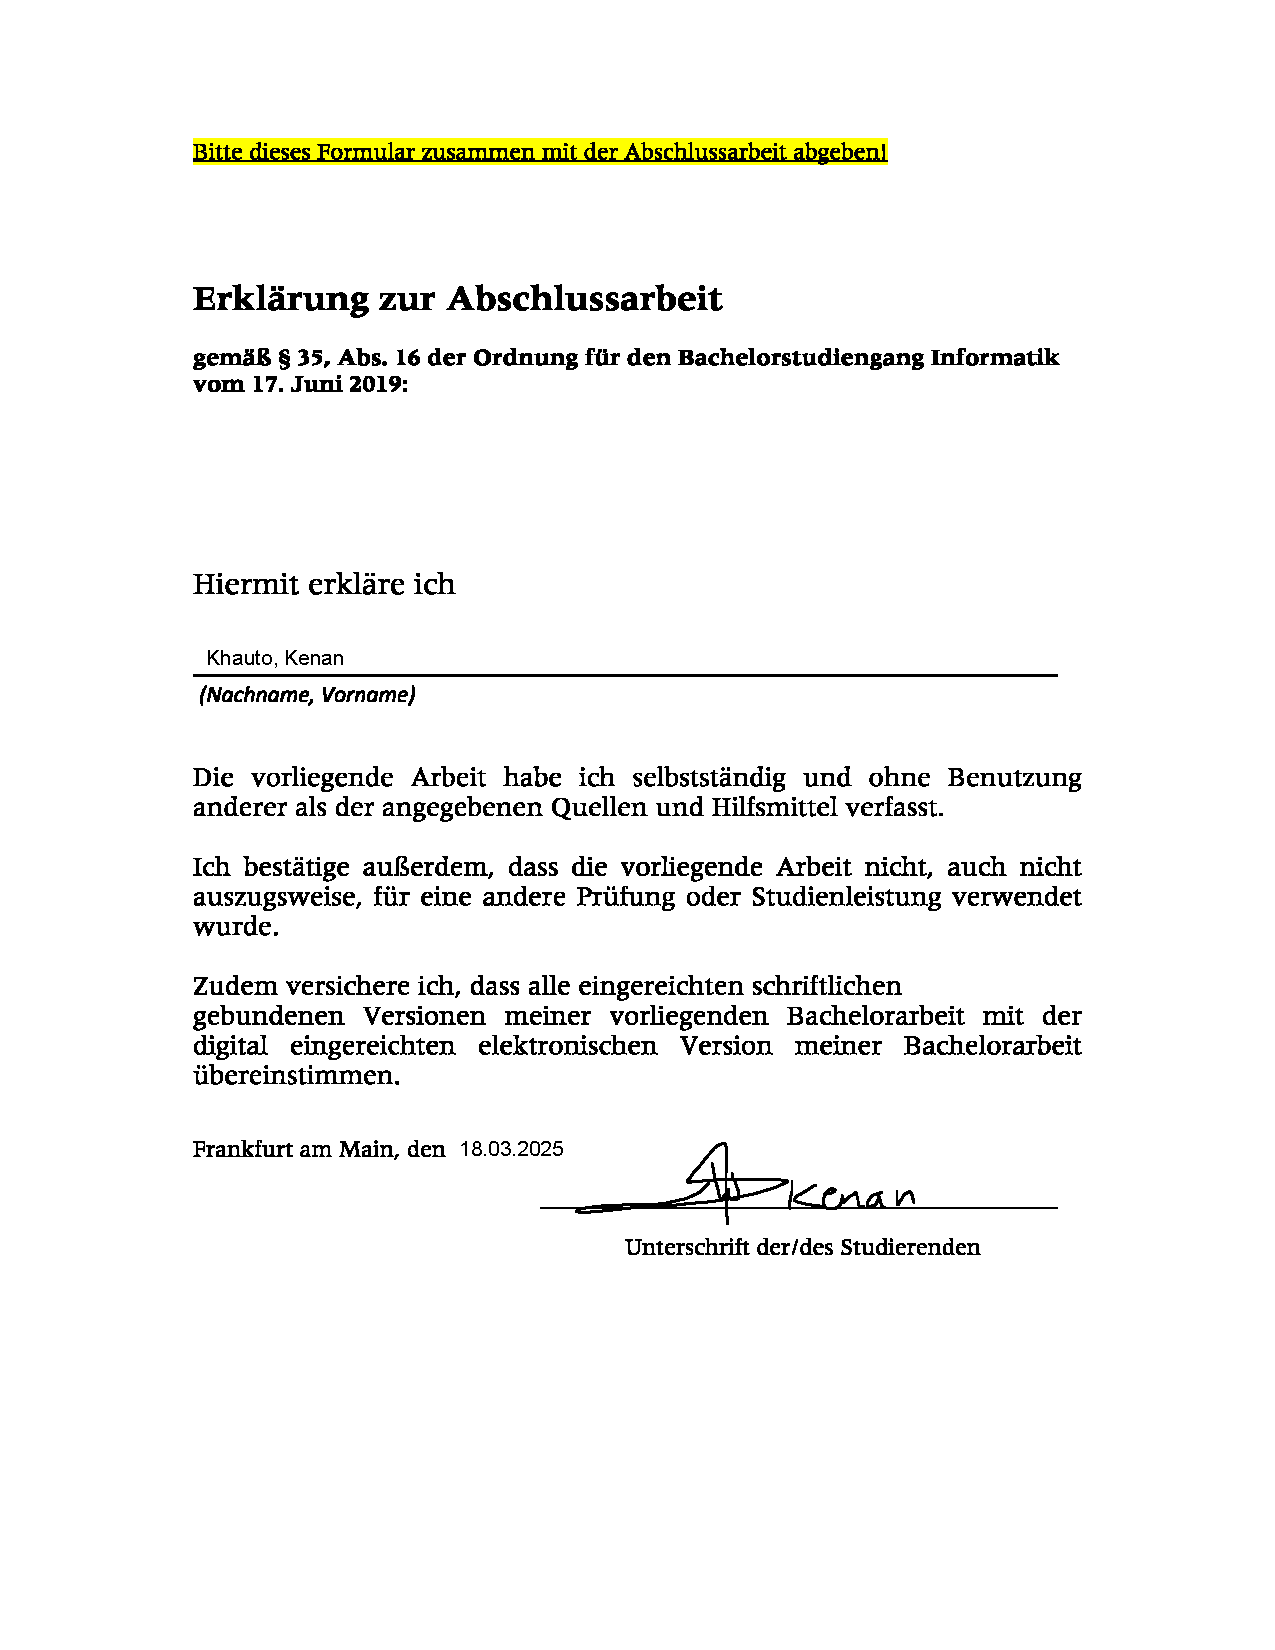
\includepdf[pages=-]{erklaerung_unterschrieben.pdf}

\tableofcontents

\chapter{Introduction}
Numismatics, the study of coins and currency, plays a crucial role in understanding the economic, political, and artistic developments 
of past civilizations \parencite{numismaticnews2023grading}. 
However, one of the biggest challenges numismatists face is the accurate classification and comparison of ancient coins, particularly 
those from early civilizations such as the Celts. Unlike modern coins with well-documented minting processes, ancient coins often lack 
standardized inscriptions, making it difficult to categorize them using traditional methods \parencite{oldcurrencyexchange2016grading}.

Traditionally, numismatists rely on expert analysis to compare coins based on their visual attributes, including shape, size, 
material, and engraving details. This process is highly time-consuming and susceptible to 
human subjectivity \parencite{numismaticnews2023biases}. Additionally, coins that have been worn down over time due to 
circulation and environmental conditions further complicate classification efforts \parencite{oldcurrencyexchange2016grading}. 
As a result, there is a pressing need for an automated, objective approach that can accurately analyze coin similarities and group 
them accordingly.

Artificial Intelligence (AI), particularly Computer Vision, offers a transformative solution to this problem \parencite{coinsweekly2023ai}. 
By leveraging deep learning techniques, AI can extract meaningful features from coin images, allowing for more precise 
similarity detection \parencite{hinh2023numi}. This study proposes a multi-step AI-driven framework to 
aid numismatists in the classification and 
analysis of ancient coins. 

\section{The Role of AI in Numismatics: Addressing Challenges in Coin Classification}
\subsection{Challenges in Traditional Numismatic Classification}
Numismatics relies heavily on expert knowledge to classify, compare, and analyze coins based on various features such as design, 
inscriptions, weight, and metal composition. However, this traditional approach has several limitations that make it inefficient 
and sometimes inconsistent.

\subsubsection{Time-Consuming Manual Classification}
\begin{itemize}
    \item Numismatic classification typically involves historians and coin experts manually inspecting each coin and identifying key features. 
    This can take a considerable amount of time, especially when dealing with large collections (e.g., museum archives, archaeological finds).

    \item The process involves cataloging coins based on their attributes (e.g., shape, weight, mint marks, wear patterns), 
    which requires extensive expertise and experience.

    \item With thousands of coins in circulation from different time periods and regions, manual classification becomes a 
    bottleneck in research and digitization efforts.
\end{itemize}

\subsubsection{Subjectivity in Expert Analysis}
\begin{itemize}
    \item Coin classification is not always objective; different experts may categorize the same coin differently based on their interpretations.

    \item Subtle differences between coins, such as small variations in engravings or damage due to wear, may lead to inconsistent conclusions.

    \item There is also the problem of bias—some experts might prioritize certain historical factors or aesthetics over technical classifications.

    \item Disagreements between experts can make it difficult to establish universally accepted classifications, leading to fragmented and sometimes conflicting datasets.
\end{itemize}

\subsubsection{Issues with Degraded Coins}
\begin{itemize}
    \item Many ancient coins are heavily worn, corroded, or damaged due to age, environmental exposure, or prolonged use in trade.
    \item Erosion can make inscriptions unreadable, which is a major issue for identification.
    \item Some coins are partially broken, missing key features necessary for classification.
    \item Traditional numismatic methods struggle to handle these cases, as manual identification relies on visible features.
    \item Reconstruction efforts can be speculative, relying on known historical data and similar coin designs.
\end{itemize}


\subsection{How AI Enhances Coin Classification and Similarity Detection}
Artificial Intelligence, particularly Computer Vision and Machine Learning, provides solutions to these challenges by 
automating classification, reducing subjectivity, and improving analysis of degraded coins.

\subsubsection{Machine Learning Approaches for Feature Extraction}
Machine learning models can automatically learn meaningful representations of coins, 
allowing for more precise and scalable classification.
\paragraph{A. Traditional Image Processing Approaches}

\begin{itemize}
    \item Early methods relied on handcrafted features such as:
    \begin{itemize}
        \item Edge detection (Sobel~\cite{gonzalez2002digital}, Canny~\cite{canny1986edge}) to identify coin contours.
        \item Histogram of Oriented Gradients (HOG) to detect texture and shapes ~\parencite{dalal2005hog}.
        \item Scale-Invariant Feature Transform (SIFT) for keypoint matching between coins ~\parencite{lowe2004sift}.
    \end{itemize}

    \item While these techniques provided some level of automation, they lacked robustness against variations in lighting, 
    orientation, and wear.
\end{itemize}
\paragraph{B. Deep Learning-Based Feature Extraction}
\begin{itemize}
    \item {\bfseries Convolutional Neural Networks (CNNs)} revolutionized feature extraction~\parencite{lecun1998cnn} by learning hierarchical patterns in images.
    \item Instead of relying on predefined rules, CNNs automatically extract:
    \begin{itemize}
        \item Low-level features (edges, textures).
        \item Mid-level features (shapes, engravings).
        \item High-level features (mint marks, portraits, inscriptions).
    \end{itemize}

    \item Popular architectures include: \begin{itemize}
        \item {\bfseries ResNet, EfficientNet, VGG-16} for feature learning ~\parencite{he2016resnet, tan2019efficientnet, simonyan2015vgg}.
        \item {\bfseries Vision Transformers (ViTs)} for global pattern recognition ~\parencite{dosovitskiy2021vit}.
    \end{itemize}
    \item These deep models significantly outperform traditional handcrafted methods, providing robust, scalable, 
    and precise feature extraction.
\end{itemize}


\paragraph{C. Self-Supervised Learning for Coin Analysis}
\begin{itemize}
    \item {\bfseries SimCLR, BYOL, and MoCo v3} use contrastive learning to train models without labeled data~\parencite{chen2020simclr, grill2020byol, chen2021mocov3}.
    \item These methods are particularly useful for numismatics, where labeled datasets are scarce.
    \item The model learns to differentiate coins based on similarity, making it ideal for grouping similar coins even without prior knowledge.
\end{itemize}

\paragraph{Code and Reproducibility}
To ensure the reproducibility of our experiments and provide an in-depth look at the implementation, 
all code related to this study, including dataset processing, feature extraction, multimodal fusion, and network analysis, 
has been made publicly available on GitHub. 
The repository can be accessed at: \begin{small}
    \begin{center} \href{https://github.com/KenanKhauto/AI-driven-coin-analysis}{\texttt{https://github.com/KenanKhauto/AI-driven-coin-analysis}}\end{center}
\end{small}

\chapter{Dataset Overview: Source, Composition, and Preprocessing}
\section{Source and Composition}
This study is based on a dataset of numismatic images and metadata, which was kindly provided by Markus Möller, 
a master’s student at the University of Leipzig. The dataset consists of coin images along with weight, diameter, 
and other relevant details. These details were compiled by Markus from various numismatic collections, where the 
original information was typically recorded on small paper notes accompanying the coins. Some of these notes exist 
in printed form as well.

The images originate from multiple museum and private collections, which are summarized in ~\ref{tab:collection_summary}. 
The dataset does not originate from a single unified publication but was instead curated from individual coin 
collection records.

\begin{table}[H]
\centering
\caption{Summary of Numismatic Collections and Coin Counts}
\label{tab:collection_summary}
\begin{tabular}{|l|c|}
\hline
\textbf{Collection Name} & \textbf{Number of Coins} \\
\hline
Linz Neubau & 166 \\
Archäologische Staatssammlung München & 198 \\
Deggendorf, Kreisarchäologie & 4 \\
Gäubodenmuseum Straubing & 5 \\
Historisches Museum Regensburg & 68 \\
Oberösterreichisches Landesmuseum & 61 \\
Privatbesitz & 43 \\
Staatliche Münzsammlung München & 176 \\
Stadtmuseum Bad Reichenhall & 43 \\
\hline
\textbf{Total} & \textbf{764} \\
\hline
\end{tabular}
\end{table}

However, one challenge with the dataset is that the images exhibit inconsistent resolutions and aspect ratios, 
likely due to variations in imaging conditions, camera setups, and cropping differences. This inconsistency may 
introduce challenges in feature extraction and similarity computation, requiring preprocessing steps such as image 
resizing, normalization, and aspect ratio standardization to ensure uniformity in further analysis.



\begin{figure}[h]
    \centering
    \begin{minipage}{0.25\textwidth}
        \centering
        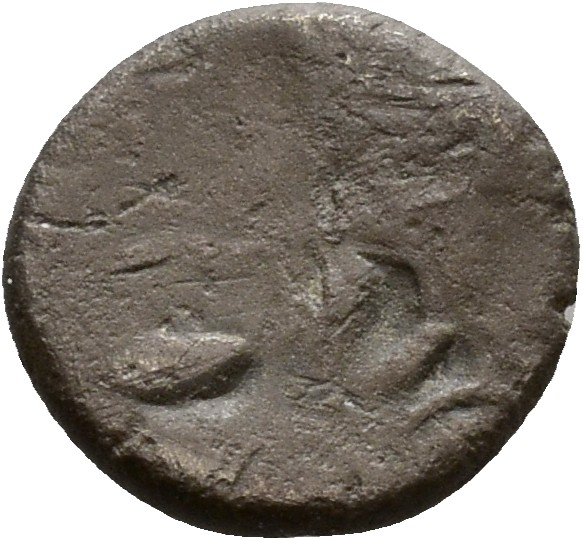
\includegraphics[width=\linewidth]{static/00012a00.jpg}
        \subcaption{Obverse of Coin 1}
    \end{minipage}
    \hfill
    \begin{minipage}{0.25\textwidth}
        \centering
        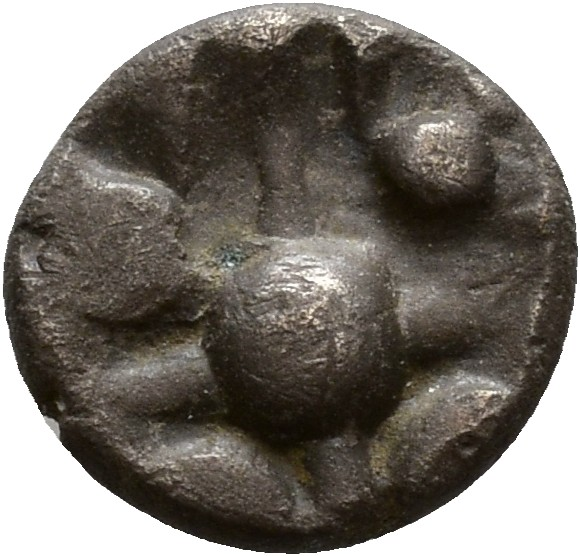
\includegraphics[width=\linewidth]{static/00012r00.jpg}
        \subcaption{Reverse of Coin 1}
    \end{minipage}

    \vspace{0.25cm}

    \begin{minipage}{0.25\textwidth}
        \centering
        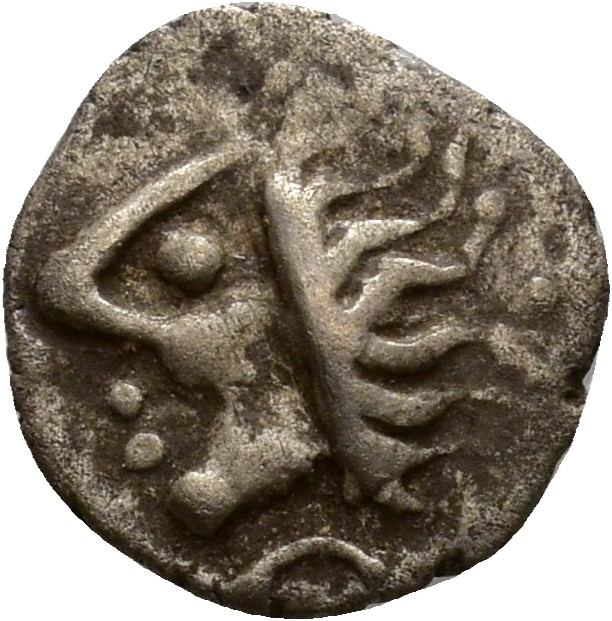
\includegraphics[width=\linewidth]{static/00016a00.jpg}
        \subcaption{Obverse of Coin 2}
    \end{minipage}
    \hfill
    \begin{minipage}{0.25\textwidth}
        \centering
        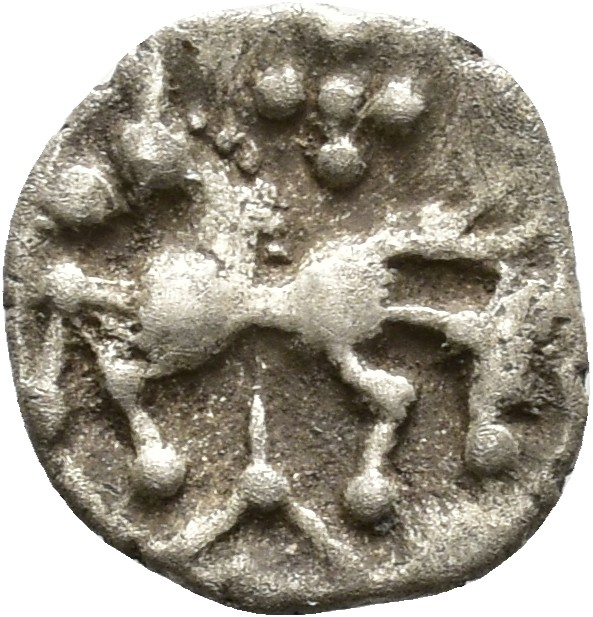
\includegraphics[width=\linewidth]{static/00016r00.jpg}
        \subcaption{Reverse of Coin 2}
    \end{minipage}

    \caption{Obverse and Reverse Views of Two Celtic Coins}
    \label{fig:coin_matrix}
\end{figure}


\section{Dataset Preprocessing}

Before applying AI-based analysis, a structured preprocessing pipeline is implemented to 
ensure consistency and quality in the dataset. The preprocessing steps include image standardization, 
pairing of obverse and reverse images, and normalization. The dataset is loaded using a custom 
\texttt{CoinDataset} class, which efficiently manages the retrieval and transformation of images.

\subsection{Handling Image Size and Resolution Inconsistencies}
One of the key challenges in the dataset is that the images exhibit varying resolutions and aspect ratios. 
To address this, each image is resized to a fixed dimension of 224×224 pixels to maintain uniform input size 
for AI models. This ensures that feature extraction remains consistent across all images. Resizing is implemented 
using the following transformation:

\begin{footnotesize}
\begin{verbatim}
transforms.Resize((224, 224))
\end{verbatim}  
\end{footnotesize}


\subsection{Image Normalization for Neural Networks}
Raw images contain intensity variations due to lighting conditions, camera settings, 
and background differences. To mitigate these issues, normalization is applied:
\begin{itemize}
    \item Images are converted to tensors for deep learning processing.
    \item Each pixel value is normalized using the ImageNet mean and standard deviation:
\end{itemize}

\begin{footnotesize}
\begin{verbatim}
transforms.Normalize(mean=[0.485, 0.456, 0.406], std=[0.229, 0.224, 0.225])
\end{verbatim}
\end{footnotesize}

This standardization improves model convergence and stabilizes feature extraction ~\parencite{krizhevsky2012imagenet}.

\subsection{Loading and Organizing the Dataset}
The dataset is structured into separate folders for obverse and reverse images. The \texttt{CoinDataset} class:
\begin{itemize}
    \item Extracts image paths and assigns them labels (\texttt{"obverse"} or \texttt{"reverse"}).
    \item Filters valid image formats (JPEG, PNG, BMP).
    \item Implements error handling to ensure robustness.
\end{itemize}

\subsection{Pairing Obverse and Reverse Coin Images}
Since each coin has two corresponding images (obverse and reverse), a pairing mechanism is used:
\begin{itemize}
    \item Filenames are parsed to extract a base name (e.g., removing suffixes such as \_obv or \_rev).
    \item Images are mapped into dictionaries for quick lookup.
    \item Only coins with a matching obverse and reverse image are included in the paired dataset.
\end{itemize}

The pairing process is handled using:

\begin{footnotesize}
\begin{center}
\begin{tcolorbox}[colback=gray!10, colframe=black, arc=5mm]
\begin{lstlisting}[language=Python, breaklines=true]
obverse_dict = {self._extract_base_name(img['filename']): img for img in self.obverse_images}
reverse_dict = {self._extract_base_name(img['filename']): img for img in self.reverse_images}
self.paired_images = [
        {"obverse": obverse_dict[key], "reverse": reverse_dict[key]}
        for key in obverse_dict.keys() & reverse_dict.keys()
    ]
\end{lstlisting}
\end{tcolorbox}
\end{center}
\end{footnotesize}



This step ensures that each coin is accurately represented as a two-sided entity, which is essential for similarity-based comparisons.

\subsection{Data Retrieval and Batching}
The dataset is designed to return images in different modes:
\begin{itemize}
    \item \textbf{Single Image Mode}: Returns individual images (either obverse or reverse).
    \item \textbf{Paired Mode}: Returns obverse and reverse images together for joint analysis.
\end{itemize}

The dataset supports PyTorch’s \texttt{DataLoader}, allowing batch-wise processing for efficient training. Example retrieval:

\begin{footnotesize}
\begin{verbatim}
obverse_image, reverse_image, filename_obv, filename_rev = dataset[idx]
\end{verbatim}
\end{footnotesize}


\subsection{Summary of Preprocessing Steps}

\begin{table}[h]
\centering
\begin{tabular}{|l|l|}
\hline
\textbf{Step}            & \textbf{Purpose} \\
\hline
Resizing (224×224)       & Standardizes image dimensions \\
Normalization            & Ensures uniform pixel value distribution \\
Loading and Filtering    & Organizes images into structured datasets \\
Pairing                 & Matches obverse and reverse images \\
Data Retrieval          & Returns images in required format\\
\hline
\end{tabular}
\caption{Preprocessing steps applied to the dataset.}
\label{tab:preprocessing}
\end{table}

These steps ensure that the dataset is structured, optimized for AI-based processing, 
and ready for similarity computations and graph-based analysis.

\chapter{Feature Extraction and Multimodal Embeddings}

\section{Feature Extraction Using Pretrained ResNet-50}

\subsection{Introduction to Feature Extraction}
Feature extraction is a crucial step in computer vision tasks, where a deep learning model converts raw image 
data into a meaningful numerical representation (embedding). These feature representations allow efficient comparison 
and clustering of images based on similarity. In this study, we utilize a \textbf{pretrained ResNet-50 model} to extract 
high-dimensional feature vectors from the obverse and reverse images of Celtic coins.

ResNet-50, a deep residual convolutional neural network, has demonstrated \textbf{state-of-the-art performance} in various 
computer vision applications~\parencite{he2016resnet}. 
By leveraging a model pre-trained on the \textbf{ImageNet dataset}~\parencite{deng2009imagenet}, 
we can benefit from features learned from millions of images, enabling \textbf{better generalization} 
even on historical numismatic images.

\subsection{Feature Extraction Pipeline}
The feature extraction process consists of the following steps:
\begin{enumerate}
    \item \textbf{Load a Pretrained ResNet-50 Model}: The final fully connected (FC) layer is removed, keeping only the convolutional feature extractor.
    \item \textbf{Process Each Coin Image (Obverse/Reverse)}: Images are passed through the network to generate embeddings.
    \item \textbf{Extract and Store Features}: The extracted feature vectors are saved for later similarity computation.
\end{enumerate}

\subsubsection{ResNet-50 as a Feature Extractor}
ResNet-50 is a \textbf{50-layer deep convolutional network} with \textbf{residual connections}, 
designed to mitigate the vanishing gradient problem in deep learning~\parencite{he2016resnet}. 
Instead of training a network from scratch, we \textbf{remove the classification layer} and use the network 
as a \textbf{fixed feature extractor}. 
Given an input image \( I \), the model outputs a \textbf{2048-dimensional feature vector} \( F(I) \):

\begin{equation}
F(I) = \text{ResNet-50}(I) \in \mathbb{R}^{2048}
\end{equation}

In the implementation, the following code initializes the ResNet-50 model and removes the final layer:

\begin{footnotesize}
\begin{lstlisting}[language=Python, frame=single, breaklines=true]
model = models.resnet50(pretrained=True)
self.feature_extractor = torch.nn.Sequential(*list(model.children())[:-1])  # Remove FC layer
\end{lstlisting}
\end{footnotesize}

\noindent
\textbf{Why ResNet-50?}
\begin{itemize}
    \item \textbf{Trained on ImageNet (1.2M images, 1,000 classes)} → Extracts \textbf{generalizable image features}.
    \item \textbf{Removes need for training from scratch}, reducing computational cost.
    \item \textbf{Well-optimized architecture} with residual connections improves gradient flow.
\end{itemize}

\subsubsection{Feature Extraction Process}
To ensure efficient feature extraction, the dataset is processed in mini-batches 
using PyTorch’s \texttt{DataLoader}. Each batch of images is:
\begin{enumerate}
    \item \textbf{Loaded into the model} (with \texttt{torch.no\_grad()} to disable gradient computation).
    \item \textbf{Passed through the feature extractor}, producing a \textbf{2048-dimensional feature vector} per image.
    \item \textbf{Stored in .npy files} for later retrieval.
\end{enumerate}

The full extraction pipeline is implemented as follows:

\begin{footnotesize}
\begin{lstlisting}[language=Python, frame=single, breaklines=true]
with torch.no_grad():
    for data in dataloader:
        images, batch_filenames = data
        images = images.to(self.device)

        # Extract features
        batch_features = self.feature_extractor(images).squeeze(-1).squeeze(-1)

        # Store results
        features.extend(batch_features.tolist())
        filenames.extend(batch_filenames)
\end{lstlisting}
\end{footnotesize}
The extracted features are then \textbf{saved as NumPy arrays (\texttt{features.npy})}, 
while filenames are stored separately in text files (\texttt{filenames.txt}). 
This allows efficient retrieval without recomputing the embeddings.

\noindent
\textbf{Standardizing Extracted Features:}
Feature standardization is a widely used preprocessing step in machine learning~\parencite{bishop2006pattern}. 
In this study, we use \texttt{StandardScaler}, a well-established normalization technique from 
the \texttt{scikit-learn} library~\parencite{scikit-learn}. This method ensures that feature distributions 
are centered at zero with unit variance, improving numerical stability.
  
After extracting ResNet-50 embeddings, the feature values are standardized using 
\texttt{StandardScaler} to ensure zero mean and unit variance. The transformation is applied as follows:

\begin{footnotesize}
\begin{lstlisting}[language=Python, frame=single, breaklines=true]
from sklearn.preprocessing import StandardScaler
        
# Load feature vectors (excluding filenames)
features_ = data.iloc[:, 1:].values  
        
# Apply StandardScaler
scaler = StandardScaler()
features_scaled = scaler.fit_transform(features_)
\end{lstlisting}
\end{footnotesize}

\noindent
\noindent
\textbf{Mathematical Definition of Standardization:}  
Feature standardization ensures that each feature has a mean of zero and a standard deviation of one. 
Given a dataset with \( n \) samples and \( d \) features, each feature \( x_j \) is standardized using:

\begin{equation}
    \tilde{x}_j = \frac{x_j - \mu_j}{\sigma_j}
\end{equation}

where:
\begin{itemize}
    \item \( \mu_j = \frac{1}{n} \sum_{i=1}^{n} x_{i,j} \) is the mean of feature \( j \).
    \item \( \sigma_j = \sqrt{\frac{1}{n} \sum_{i=1}^{n} (x_{i,j} - \mu_j)^2} \) is the standard deviation.
    \item \( \tilde{x}_j \) is the transformed (standardized) feature value.
\end{itemize}

This transformation ensures that all features are on a comparable scale, 
preventing high-magnitude features from dominating distance-based similarity calculations. 
It is particularly useful when applying clustering algorithms or computing similarity scores based on Euclidean distances.


\subsubsection{Handling Paired Images (Obverse and Reverse)}
Since each coin has \textbf{two corresponding images} (obverse and reverse), the dataset allows feature extraction for:
\begin{itemize}
    \item \textbf{Individual images} (obverse or reverse alone).
    \item \textbf{Paired images} (extracting features for both obverse and reverse in a single pass).
\end{itemize}

For paired images, the extraction pipeline processes \textbf{both images simultaneously}, 
ensuring that the corresponding obverse and reverse embeddings are stored together:

\begin{footnotesize}
\begin{lstlisting}[language=Python, frame=single, breaklines=true]
if self.label == "paired":
    obverse_features = self.feature_extractor(obverse_images).squeeze(-1).squeeze(-1)
    reverse_features = self.feature_extractor(reverse_images).squeeze(-1).squeeze(-1)
    features.extend(obverse_features.tolist() + reverse_features.tolist())
    filenames.extend(obverse_filenames + reverse_filenames)
\end{lstlisting}
\end{footnotesize}

This ensures that similarity computations can consider both views of the coin.

\subsection{Visualization of Feature Extraction}
To better understand the structure of the extracted feature embeddings, 
we apply t-Distributed Stochastic Neighbor Embedding (t-SNE) \cite{van2008visualizing} to visualize 
high-dimensional features in a 2D space. 

t-SNE is particularly useful for observing local similarities between data points. 
If the extracted features are meaningful, we expect coins with similar visual structures to form clusters in the 2D projection.

\paragraph{t-SNE Visualization for RGB Features}
\begin{figure}[H]
    \centering
    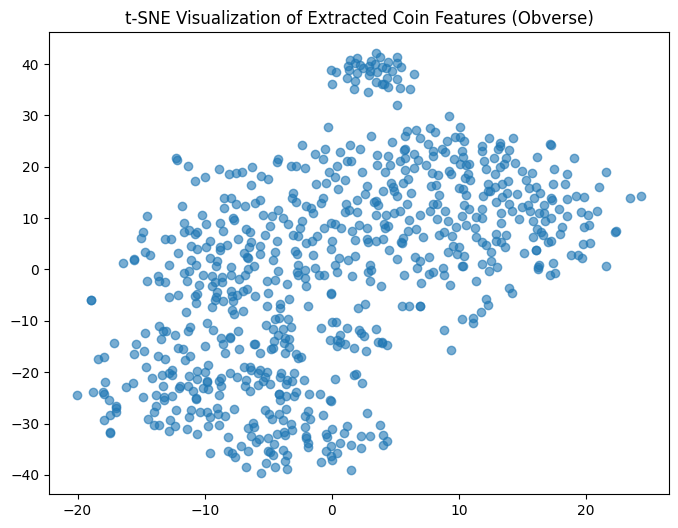
\includegraphics[width=0.7\textwidth]{static/tsne_ob_rgb.png}
    \caption{t-SNE visualization of RGB-based obverse coin features.}
    \label{fig:rgb_obverse_tsne}
\end{figure}

\begin{figure}[H]
    \centering
    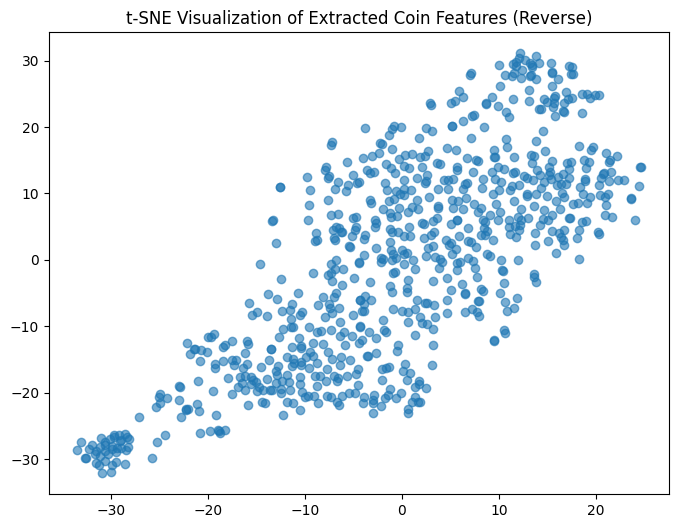
\includegraphics[width=0.7\textwidth]{static/tsne_rev_rgb.png}
    \caption{t-SNE visualization of RGB-based reverse coin features.}
    \label{fig:rgb_reverse_tsne}
\end{figure}

The RGB-based feature embeddings show a widely spread structure. Notably, 
the reverse side exhibits a more continuous distribution, suggesting that these features capture 
a greater degree of similarity compared to the obverse side.

\paragraph{t-SNE Visualization for Grayscale Features}
\begin{figure}[H]
    \centering
    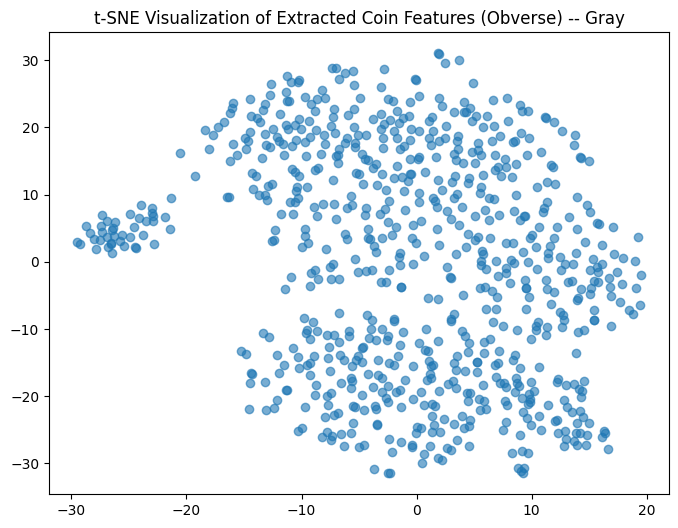
\includegraphics[width=0.7\textwidth]{static/tsne_ob_gray.png}
    \caption{t-SNE visualization of grayscale-based obverse coin features.}
    \label{fig:gray_obverse_tsne}
\end{figure}

\begin{figure}[H]
    \centering
    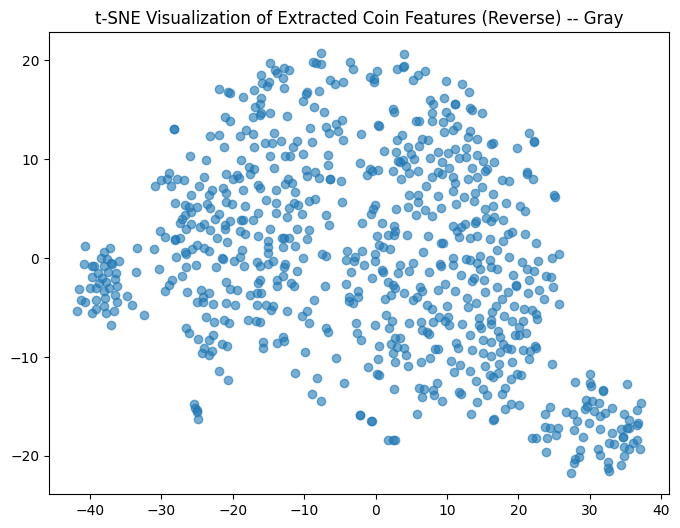
\includegraphics[width=0.7\textwidth]{static/tsne_rev_gray.png}
    \caption{t-SNE visualization of grayscale-based reverse coin features.}
    \label{fig:gray_reverse_tsne}
\end{figure}

Removing color information results in a more compact structure in the t-SNE visualization. 
This suggests that color introduces variability that is not necessarily useful for similarity detection.

\paragraph{Comparison and Implications}
The comparison between RGB and grayscale feature distributions is summarized in Table \ref{tab:tsne_comparison}.

\begin{table}[H]
    \centering
    \begin{tabular}{|c|c|c|}
        \hline
        Feature & RGB t-SNE & Grayscale t-SNE \\
        \hline
        Cluster Separation & More dispersed & More compact \\
        Feature Diversity & Higher due to color differences & Lower, focused on structure \\
        Obverse Distribution & Wider spread & More structured \\
        Reverse Distribution & Semi-structured & Highly structured \\
        \hline
    \end{tabular}
    \caption{Comparison of RGB vs. Grayscale t-SNE Distributions}
    \label{tab:tsne_comparison}
\end{table}

These results suggest that grayscale embeddings may provide better structured similarity representations, 
which could improve similarity search and clustering in later stages.


The following Python code generates a t-SNE visualization:

\begin{footnotesize}
\begin{lstlisting}[language=Python, frame=single, breaklines=true]
from sklearn.manifold import TSNE
import matplotlib.pyplot as plt

features, filenames = extractor.load_features("features.npy", "filenames.txt")

# Reduce to 2D using t-SNE
tsne = TSNE(n_components=2, perplexity=30, random_state=42)
features_2d = tsne.fit_transform(features)

# Plot
plt.figure(figsize=(8, 6))
plt.scatter(features_2d[:, 0], features_2d[:, 1], alpha=0.6)
plt.title("t-SNE Visualization of Extracted Coin Features")
plt.show()
\end{lstlisting}
\end{footnotesize}

\subsection{Summary of Feature Extraction}
\begin{table}[h]
\centering
\begin{tabular}{|l|l|}
\hline
\textbf{Step}            & \textbf{Description} \\
\hline
ResNet-50 Model        & Pretrained on ImageNet (final layer removed) \\
Feature Size           & 2048-dimensional vector per image \\
Batch Processing       & Uses mini-batches for efficient extraction \\
Paired Image Handling  & Processes obverse \& reverse together \\
Storage Format         & Saves embeddings in \texttt{.npy} files \\
\hline
\end{tabular}
\caption{Summary of feature extraction steps.}
\label{tab:feature_extraction}
\end{table}


\section{Multimodal Feature Extraction: Combining Image and Text}
\label{sec:multimodal_feature_extraction}

The classification and analysis of ancient coins involve both \textbf{visual} and \textbf{textual} information. 
The obverse and reverse sides of coins feature symbols, inscriptions, and patterns that are crucial for identification. 
In this section, we describe how image and text features are extracted separately and then fused using a \textbf{multimodal learning approach}.

\subsection{Processing the Dataset}
\label{subsec:processing_dataset}
In a previous chapter, we described the initial preprocessing steps applied to the dataset. 
However, in this section, we focus on an additional processing step necessary for obtaining the \textbf{categories} (types) of the images. 

The dataset consists of images stored in a structured folder system. The main dataset folder contains multiple subfolders, 
where each subfolder represents a specific category or type of coin imagery. The name of each subfolder corresponds to the 
type of images it contains. Some example categories include:

\begin{itemize}
    \item \textbf{Kopf mit großem Auge} (Head with Large Eye)
    \item \textbf{Magdalensberg} 
    \item \textbf{Karlstein}
\end{itemize}

Each image inside a subfolder inherits the category of that subfolder. 
However, not all images are stored within these categorized subfolders. 
Some images remain in the main dataset directory without any assigned category, 
meaning they are \textbf{unclassified}. This presents a challenge, 
as we need a strategy to handle these unclassified images appropriately.

To address this issue, we introduce a solution in a later subsection where 
we discuss \textbf{CLIP-based text embeddings}\parencite{radford2021learning}. 
Specifically, we will define textual templates that allow us to generate meaningful embeddings for 
both categorized and uncategorized images. 

The implementation of this dataset processing logic is integrated into the \texttt{CoinDataset} 
class within the \texttt{image\_loader.py} file. This class automatically associates each image with its corresponding category 
if available, while also tracking images that lack classification.


\subsection{Introduction to CLIP}

Contrastive Language-Image Pretraining (CLIP) is a \textbf{multimodal neural network}
developed by OpenAI \cite{radford2021learning}. It is designed to learn joint 
representations of \textbf{images and text} through contrastive learning, enabling zero-shot learning on a wide range of 
visual recognition tasks. Unlike traditional supervised learning approaches, which require labeled datasets for each 
specific task, CLIP generalizes across domains by leveraging large-scale internet data.

\subsubsection{How CLIP Works}

CLIP consists of two separate neural networks:
\begin{enumerate}
    \item A \textbf{Vision Encoder}, typically a convolutional neural network (CNN) such as ResNet-50 or 
    a Vision Transformer (ViT), which converts images into fixed-dimensional feature vectors.
    \item A \textbf{Text Encoder}, usually a transformer-based model, which encodes textual descriptions into 
    feature vectors of the same dimension as the image embeddings.
\end{enumerate}

During training, CLIP is presented with \textbf{image-text pairs}. The model learns to project similar images and textual 
descriptions closer together in a shared embedding space while pushing dissimilar pairs further apart. 
This is achieved using a contrastive loss function.

\begin{figure}[h]
    \centering
    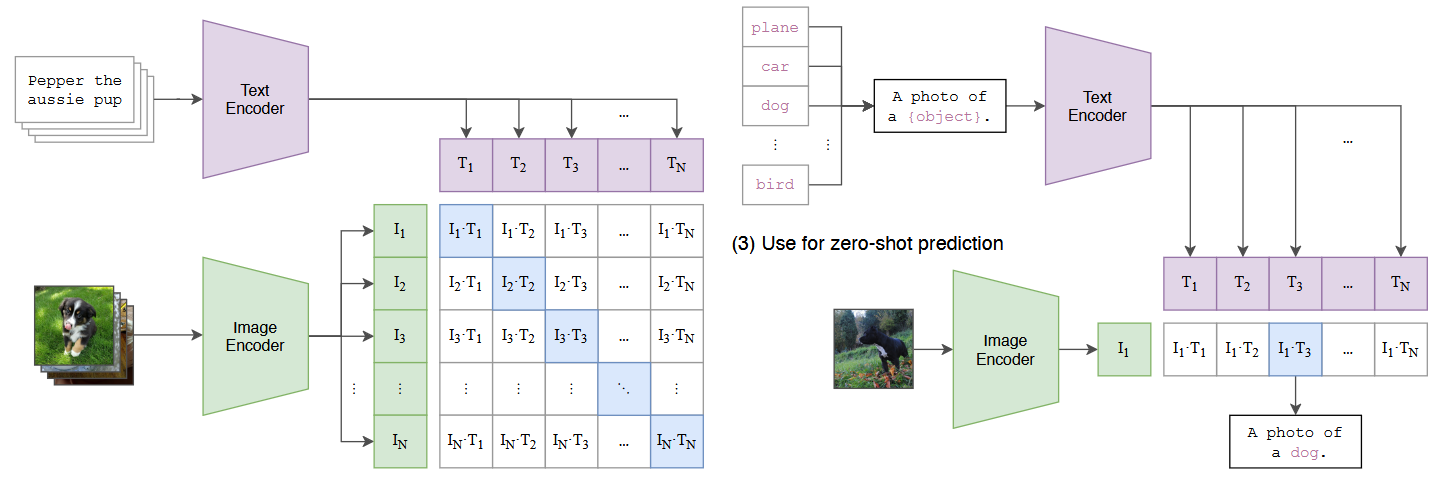
\includegraphics[width=0.8\textwidth]{static/clip_arch.png}
    \caption{Illustration of CLIP’s architecture, showing how image and text embeddings are mapped into a shared feature space \parencite{radford2021learning}.}
    \label{fig:clip_architecture}
\end{figure}

\subsubsection{Why CLIP is Useful for our Study}

Traditional image classification models rely on predefined labels and require fine-tuning for each new dataset. 
However, CLIP enables a \textbf{more flexible and generalizable} approach. Instead of explicitly training a model to 
recognize specific coin types, we can use text prompts to describe coin features and let CLIP generate meaningful feature representations.

This capability is particularly valuable in numismatics, where:
\begin{itemize}
    \item Some coins may not be labeled in the dataset (as discussed in ~\ref{subsec:processing_dataset}).
    \item Many coin images share visual similarities but differ in textual descriptions.
    \item There exists a rich historical and semantic context that cannot be fully captured by visual features alone.
\end{itemize}

By leveraging CLIP, we can extract both image and text embeddings, which we later fuse using a \textbf{Multilayer Perceptron (MLP)}. 
This fusion enhances similarity measurements by integrating multimodal features.

\subsubsection{Zero-Shot Learning with CLIP}

One of CLIP’s most powerful features is \textbf{zero-shot learning}. 
Because CLIP was trained on large-scale internet data, it can classify images \textbf{without requiring labeled training data}
for every category. This means that even if a specific coin type was never explicitly trained, 
CLIP can still recognize similarities based on textual descriptions.

For example, if we describe a coin as "\textit{A Roman coin with a laurel wreath}" and compare it to a 
database of coin images, CLIP will retrieve the most visually and semantically relevant matches.

\subsubsection{Challenges and Limitations of CLIP}

While CLIP provides powerful capabilities, it also has limitations:
\begin{itemize}
    \item It relies heavily on \textbf{pretrained knowledge} and may not recognize rare or highly specialized 
    numismatic features that are not well-represented in internet data.
    \item The text embeddings' quality depends on \textbf{well-crafted textual prompts}.
    \item CLIP does not perform \textbf{fine-grained coin classification} as accurately as models trained on domain-specific datasets.
\end{itemize}

Despite these challenges, CLIP serves as a \textbf{strong foundation} for our multimodal feature extraction approach. 
In the next subsection, we discuss how we generate textual templates to obtain meaningful text embeddings for coin classification.


\subsection{Creating Text Embeddings Using Templates}

In order to leverage the power of CLIP for multimodal representation learning, we need to generate meaningful 
textual descriptions that align well with the image representations. 
CLIP maps both images and text into a \textbf{shared embedding space}, which means that the quality of the textual descriptions 
directly impacts how well the textual and visual representations align. 
Instead of using simple class labels, we construct rich textual prompts to enhance the expressiveness of our text embeddings.

\subsubsection{The Importance of Text Prompts}

The quality of text embeddings in CLIP depends heavily on how well the descriptions capture the \textbf{semantic meaning} of 
the corresponding images. A direct mapping using single-word class labels such as \textit{"Magdalensberg"} or \textit{"Karlstein"} 
would not fully utilize CLIP’s ability to generalize. Instead, template-based descriptions provide contextualized representations 
that improve feature alignment between modalities.

To generate meaningful textual representations for our dataset, we define structured text templates based on whether the image 
belongs to the \textbf{obverse} or \textbf{reverse} side of a coin.

\subsubsection{Text Template Design}

Given that coin images often depict symbolic and historical figures, we introduce structured text templates. 
The templates dynamically adjust based on the type of coin and the side (obverse or reverse) of the image. 
The key idea is to create natural language descriptions that provide CLIP with semantic context while maintaining generalizability.

\begin{itemize}
    \item For coins with known types, we describe them using:
    \begin{quote}
        \textit{"This is the \textbf{[side]} of an ancient Celtic coin depicting \textbf{[type]}."}
    \end{quote}
    \item For coins without assigned types (unknown class), we use a more general template:
    \begin{quote}
        \textit{"The \textbf{[side]} of this ancient Celtic coin has an unidentified design."}
    \end{quote}
\end{itemize}

By structuring our textual inputs in this way, we ensure that the model learns generalizable textual representations for coins while 
still allowing fine-grained differentiation.

\subsubsection{Implementation of Text Templates}

The following Python function dynamically generates textual descriptions based on the coin’s category and side:

\begin{footnotesize}
\begin{center}
\begin{tcolorbox}[colback=gray!10, colframe=black, arc=5mm]
\begin{lstlisting}[language=Python, breaklines=true]

def generate_text_description(side, coin_type):
"""
Generates a textual description for CLIP embedding.
:param side: "obverse" or "reverse".
:param coin_type: The type of the coin (or "Unknown").
:return: Formatted text description.
"""
if coin_type.lower() == "unknown":
    return f"The {side} of this ancient Celtic coin has an unidentified design."
else:
    return f"This is the {side} of an ancient Celtic coin depicting {coin_type}."

\end{lstlisting}
\end{tcolorbox}
\end{center}
\end{footnotesize}

This function is applied to each sample in the dataset before feeding it into CLIP’s \textbf{text encoder}. 
In the next subsection, we describe how we use CLIP to extract both image and text embeddings.

\subsection{Extracting Features with CLIP}

After defining meaningful text templates, we extract \textbf{multimodal feature embeddings} using OpenAI’s CLIP model. 
CLIP consists of two separate encoders:
\begin{itemize}
    \item \textbf{A Vision Encoder:} A Vision Transformer (ViT-B/32) that converts images into image embeddings.
    \item \textbf{A Text Encoder:} A transformer-based model that converts descriptions into text embeddings.
\end{itemize}

Both encoders map their respective inputs into a \textbf{shared embedding space}, enabling cross-modal comparisons 
between images and text.

\subsubsection{Embedding Extraction Pipeline}

The CLIP model processes batches of images and text descriptions simultaneously, 
computing embeddings for each. The full extraction pipeline is as follows:

\begin{enumerate}
    \item Load the dataset containing obverse and reverse coin images.
    \item Preprocess the images using CLIP’s built-in image preprocessing pipeline.
    \item Tokenize the dynamically generated text prompts using CLIP’s text tokenizer.
    \item Pass both the images and the text prompts through the corresponding CLIP encoders.
    \item Store the extracted embeddings for further processing.
\end{enumerate}

\subsubsection{Implementation of CLIP-Based Feature Extraction}

The following Python Code extracts both image and text embeddings from the dataset using CLIP:

\begin{footnotesize}
\begin{center}
\begin{tcolorbox}[colback=gray!10, colframe=black, arc=5mm]
\begin{lstlisting}[language=Python, breaklines=true]
def extract_embeddings(self):
    """
    Extracts both text and image embeddings from the dataset.
    :return: Lists of image embeddings, text embeddings, filenames.
    """
    dataloader = DataLoader(self.dataset, batch_size=self.batch_size, shuffle=False)
    image_embeddings, text_embeddings, filenames, base_text = [], [], [], []

    with torch.no_grad():
        for batch in dataloader:
            images, batch_filenames, batch_types, batch_labels = batch

            # Convert images to CLIP format
            images = images.to(self.device)

            # Generate text descriptions dynamically
            text_descriptions = [self.generate_text_description(label, ctype) 
                                    for ctype, label in zip(batch_types, batch_labels)]

            # Compute text and image embeddings
            text_tokens = clip.tokenize(text_descriptions).to(self.device)
            text_emb = self.model.encode_text(text_tokens)
            image_emb = self.model.encode_image(images)

            # Store embeddings and filenames
            image_embeddings.extend(image_emb.cpu().numpy())
            text_embeddings.extend(text_emb.cpu().numpy())
            filenames.extend(batch_filenames)
            base_text.extend(text_descriptions)

    return image_embeddings, text_embeddings, filenames, base_text
\end{lstlisting}
\end{tcolorbox}
\end{center}
\end{footnotesize}

This implementation ensures that both image and text embeddings are computed efficiently in batches.

With CLIP embeddings extracted, the next step is to \textbf{fuse} them using a \textbf{Multilayer Perceptron (MLP)}. 
The fusion process is covered in the subsequent section.

\subsection{Fusion Using an MLP}

After extracting separate embeddings for images and text using CLIP, the next step is to 
combine them into a unified multimodal representation. We achieve this by using a \textbf{Multilayer Perceptron (MLP)}, 
which learns to integrate the information from both modalities into a \textbf{single feature space}. 
This fusion enables improved similarity computations, as it allows the model to capture both visual and textual characteristics in 
a shared representation.

\subsubsection{What is a Multilayer Perceptron (MLP)?}

A \textbf{Multilayer Perceptron (MLP)} is a type of artificial neural network that consists of 
multiple layers of fully connected neurons. 
Each neuron applies a weighted sum of its inputs, followed by a non-linear activation function \parencite{goodfellow2016deep}. 
The fundamental components of an MLP are:

\begin{itemize}
    \item \textbf{Input Layer:} Receives the input features (in our case, concatenated image and text embeddings).
    \item \textbf{Hidden Layers:} Transform the input using linear transformations followed by non-linear activation functions (e.g., ReLU).
    \item \textbf{Output Layer:} Produces the final fused embedding, representing both image and text features.
\end{itemize}

In our model, the input to the MLP is a concatenation of the CLIP image and text embeddings. 
The network learns a compressed feature representation that effectively combines information from both modalities.

\subsubsection{Architecture of the Fusion Network}

The MLP fusion network takes 512-dimensional image embeddings and 512-dimensional text embeddings, 
concatenates them into a 1024-dimensional vector, and processes them through two fully connected layers:

\begin{itemize}
    \item \textbf{First Layer (Fully Connected)}: Projects the 1024-dimensional input into a lower-dimensional 256-dimensional space.
    \item \textbf{Activation Function (ReLU)}: Applies non-linearity to enable the network to learn complex relationships.
    \item \textbf{Second Layer (Fully Connected)}: Maps the 256-dimensional hidden representation to a final 128-dimensional multimodal embedding.
\end{itemize}

The final 128-dimensional fused embedding is used for similarity computations and further analysis.

\begin{footnotesize}
\begin{center}
\begin{tcolorbox}[colback=gray!10, colframe=black, arc=5mm]
\begin{lstlisting}[language=Python, breaklines=true]
import torch
import torch.nn as nn

class MLPFusion(nn.Module):
    def __init__(self, input_dim=512, hidden_dim=256, output_dim=128):
        """
        MLP-based fusion of CLIP image and text embeddings.
        :param input_dim: Input feature dimension (512 for CLIP ViT-B/32).
        :param hidden_dim: Hidden layer size.
        :param output_dim: Output embedding size after fusion.
        """
        super(MLPFusion, self).__init__()

        self.fc1 = nn.Linear(input_dim * 2, hidden_dim)  # Concatenate img + text embeddings
        self.relu = nn.ReLU()
        self.fc2 = nn.Linear(hidden_dim, output_dim)  # Project to shared space

    def forward(self, img_emb, txt_emb):
        """
        Forward pass to fuse image and text embeddings.
        :param img_emb: Image embedding tensor (batch_size, 512).
        :param txt_emb: Text embedding tensor (batch_size, 512).
        :return: Fused embedding (batch_size, output_dim).
        """
        x = torch.cat((img_emb, txt_emb), dim=1)  # Concatenate embeddings
        x = self.relu(self.fc1(x))
        x = self.fc2(x)
        return x  # Return fused representation
\end{lstlisting}
\end{tcolorbox}
\end{center}
\end{footnotesize}

\subsubsection{Loss Function for Multimodal Fusion}

To train the fusion model effectively, we use Cosine Embedding Loss. 
This loss function ensures that similar image-text pairs are pulled closer together, while dissimilar pairs 
are pushed further apart in the embedding space.

\textbf{Cosine Similarity} measures how similar two vectors are, based on the angle between them:

\[
\text{Cosine Similarity} = \frac{A \cdot B}{||A|| ||B||}
\]

where \( A \) and \( B \) are the fused embeddings of the image and text.

The Cosine Embedding Loss is defined as:

\[
L = \begin{cases}
1 - \cos(A, B), & \text{if labels are similar} \\
\max(0, \cos(A, B)), & \text{if labels are dissimilar}
\end{cases}
\]

This ensures that embeddings from related images and texts are aligned closely in feature space \parencite{hadsell2006dimensionality}.

\begin{footnotesize}
\begin{center}
\begin{tcolorbox}[colback=gray!10, colframe=black, arc=5mm]
\begin{lstlisting}[language=Python, breaklines=true]
class FusionLoss(nn.Module):
    def __init__(self):
        super(FusionLoss, self).__init__()
        self.cosine_loss = nn.CosineEmbeddingLoss()

    def forward(self, fused_img, fused_txt, labels):
        """
        Compute contrastive loss for multimodal fusion.
        :param fused_img: Fused image embeddings.
        :param fused_txt: Fused text embeddings.
        :param labels: 1 for matching pairs, -1 for non-matching pairs.
        """
        return self.cosine_loss(fused_img, fused_txt, labels)
\end{lstlisting}
\end{tcolorbox}
\end{center}
\end{footnotesize}

\subsubsection{Final Fused Embedding Dimension}

The final output of the fusion model is a 128-dimensional feature vector. 
This compressed representation is a rich multimodal encoding that integrates both visual and textual information about the coin.

\begin{itemize}
    \item The \textbf{image} contributes information about the coin’s shape, texture, and engravings.
    \item The \textbf{text} adds semantic meaning related to coin history and category.
\end{itemize}

By merging these modalities, we improve similarity computations and provide a more robust feature space for coin classification.



\subsection{t-SNE Visualization of Fused Features}
In order to gain insights into the effectiveness of our multimodal fusion, 
we apply \textbf{t-Distributed Stochastic Neighbor Embedding (t-SNE)} to the fused embeddings \parencite{van2008visualizing}. 
This allows us to visually assess whether the fused embeddings exhibit meaningful clusters,
which would indicate that the model is learning useful representations of the coins.

Figure \ref{fig:tsne_obverse} and \ref{fig:tsne_reverse} show the t-SNE projection of the fused image-text embeddings 
for both obverse and reverse coin sides.

\begin{figure}[H]
    \centering
    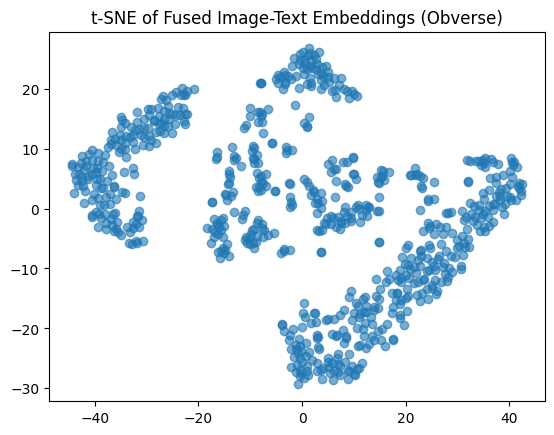
\includegraphics[width=0.8\textwidth]{static/tsne_ob_fused.png}
    \caption{t-SNE Visualization of Fused Image-Text Embeddings for Obverse Coins.}
    \label{fig:tsne_obverse}
\end{figure}

\begin{figure}[H]
    \centering
    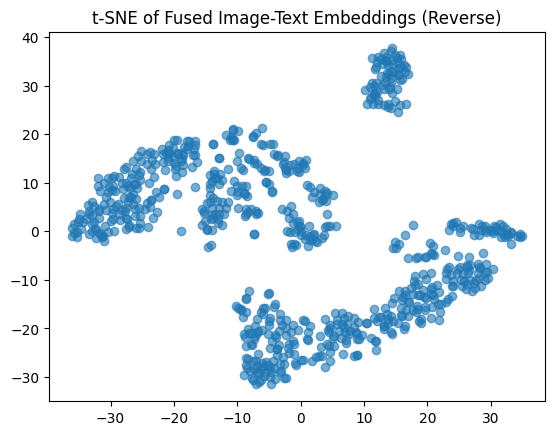
\includegraphics[width=0.8\textwidth]{static/tsne_rev_fused.png}
    \caption{t-SNE Visualization of Fused Image-Text Embeddings for Reverse Coins.}
    \label{fig:tsne_reverse}
\end{figure}

\subsubsection{Observations}

From the visualizations, we can make the following observations:

\begin{itemize}
    \item \textbf{Formation of Clusters}: Both the obverse and reverse embeddings show distinct clusters, 
    suggesting that the multimodal fusion process successfully captures meaningful relationships between coin 
    images and their textual descriptions.
    
    \item \textbf{Separation of Coin Types}: The presence of well-defined groups indicates that similar coin types tend to 
    be mapped close together in the fused feature space. This is a strong indication that the fusion model is effectively aligning 
    the visual and textual modalities.

    \item \textbf{Potential Outliers}: In both plots, there are a few data points that are noticeably distant from the main clusters. 
    These might correspond to coins that lack clear textual descriptions or have unique features that distinguish them from the majority.
\end{itemize}

These results confirm that our approach to multimodal fusion preserves meaningful relationships between images and text 
while structuring the latent space in a way that allows for intuitive organization of different coin types.

\subsection{Summary of Multimodal Feature Extraction}
In this section, we introduced a multimodal approach to feature extraction by combining both image and textual information 
using CLIP embeddings. We began by discussing the dataset processing steps, where coin images were categorized based on their types, 
and how textual descriptions were generated dynamically using structured templates. This allowed us to create meaningful text embeddings 
that align well with the visual representations.

We then explored the methodology behind CLIP and how it enables joint vision-language learning, followed by the extraction of 
image and text features. To enhance the multimodal representation, we fused these embeddings using 
a \textbf{Multi-Layer Perceptron (MLP)}, effectively combining visual and textual information into a unified latent space. 
The fusion process was guided by a \textbf{Cosine Embedding Loss}, ensuring that corresponding image-text pairs remain close in the 
embedding space.

To evaluate the quality of the fused embeddings, we visualized them using \textbf{t-SNE}, which demonstrated meaningful 
clustering patterns, indicating that the fusion model successfully captured structural relationships between different coin types.

Our findings suggest that multimodal feature extraction enhances the ability to learn meaningful representations of ancient coins. 
This approach lays the foundation for further comparisons in the next section, where we analyze the differences in similarity 
computations between image-only embeddings and fused image-text embeddings.


\section{Computing Similarity Across Embeddings}

\subsection{Introduction to Cosine Similarity}
Cosine similarity is a widely used metric for measuring the similarity between two high-dimensional vectors. 
Given two vectors \( A \) and \( B \), the cosine similarity is computed as:

\begin{equation}
\text{cosine\_sim}(A, B) = \frac{A \cdot B}{\|A\| \|B\|}
\end{equation}

where \( A \cdot B \) represents the dot product of the two vectors, 
and \( \|A\| \) and \( \|B\| \) denote their Euclidean norms. 
This metric is particularly useful for our study because it measures the orientation between vectors rather than their magnitude, 
making it well-suited for comparing feature representations in an embedding space.

In the context of our study, we use cosine similarity to measure the similarity between:
\begin{itemize}
    \item \textbf{Image-based embeddings:} Extracted using a pretrained ResNet50 model.
    \item \textbf{Multimodal embeddings:} Obtained by fusing CLIP image and text representations through an MLP.
\end{itemize}

By comparing these embeddings, we can analyze how the fusion of textual and visual information impacts similarity retrieval.

\subsection{Measuring Similarity for Image-Based Embeddings}
For image-based embeddings, we use the feature vectors extracted from a pretrained ResNet50 model. 
These embeddings are stored in \texttt{.npy} files for both obverse and reverse sides of the coins. 

The similarity retrieval process follows these steps:
\begin{enumerate}
    \item Load the stored embeddings and their corresponding filenames.
    \item Compute the cosine similarity between a query image and all other images in the dataset.
    \item Retrieve the most and least similar images based on similarity scores.
\end{enumerate}

This process allows us to analyze how well ResNet50 features capture the \textbf{visual similarity} between coins. 
The retrieved images demonstrate how the network distinguishes between similar and dissimilar coin patterns.

\subsection{Measuring Similarity in Multimodal Space}
In contrast to image-based similarity, the multimodal approach integrates \textbf{both visual and textual features} 
to create a more enriched representation. We utilize CLIP embeddings, where:
\begin{itemize}
    \item The image embeddings are extracted from the CLIP vision encoder.
    \item The text embeddings are derived from templates describing the coin's characteristics.
    \item These two embeddings are fused using an MLP to produce a final multimodal representation.
\end{itemize}

The similarity retrieval process remains the same: cosine similarity is computed between the fused representations of a 
query coin and all others in the dataset. This method allows us to leverage textual context, potentially improving retrieval 
performance by aligning visual features with descriptive labels.

\subsection{Comparison of Results}
After computing similarity scores for both embedding types, we analyze the differences between the two approaches. 
Below are some examples illustrating the retrieved images for a given query:

\begin{figure}[H]
    \centering
    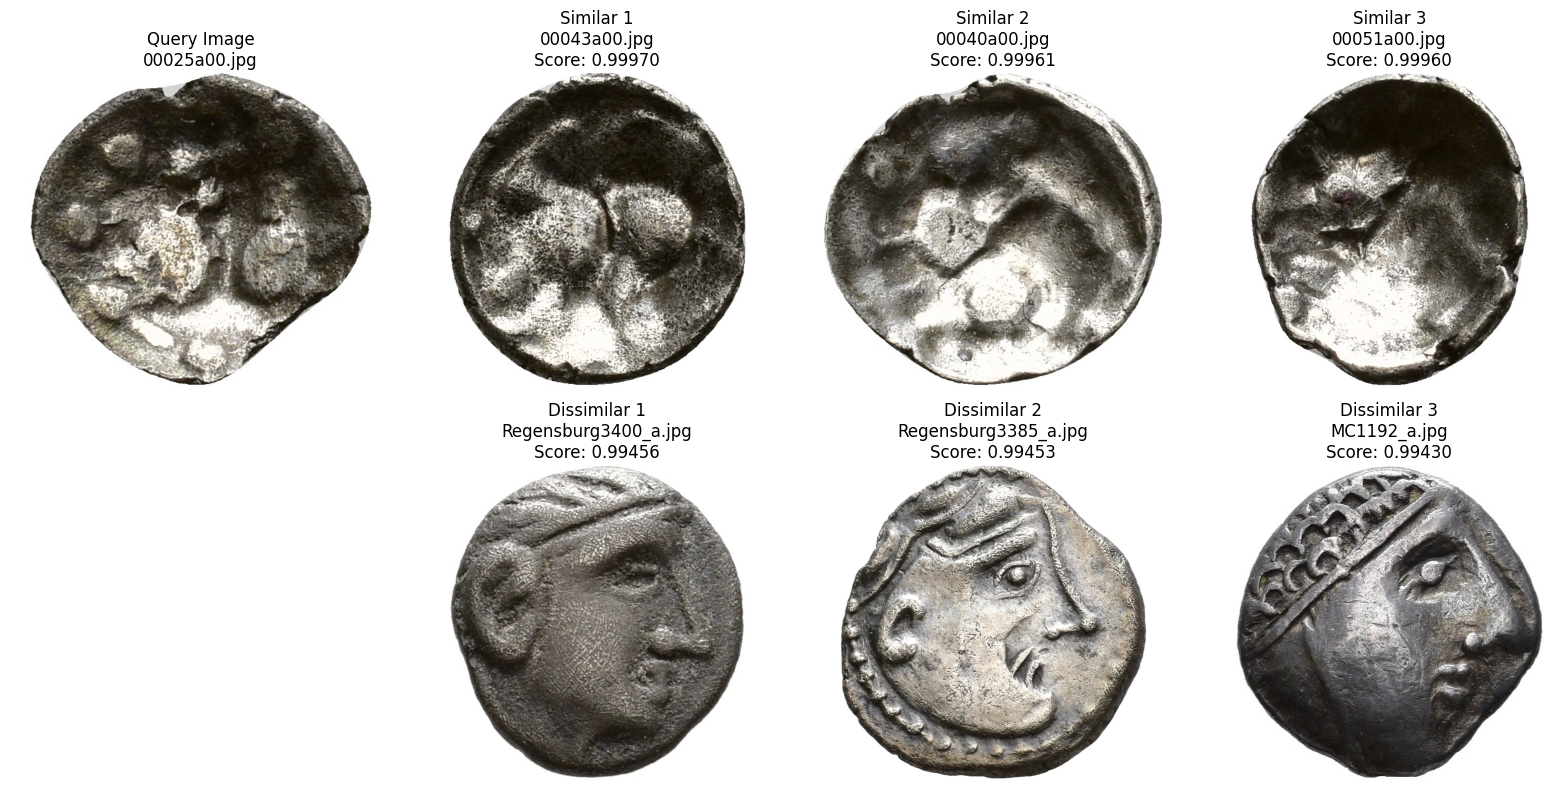
\includegraphics[width=0.8\textwidth]{static/fused_similarity_example_1.png}
    \caption{Example 1: Similarity retrieval using fused embeddings (text+image).}
    \label{fig:fused_similarity1}
\end{figure}

\begin{figure}[H]
    \centering
    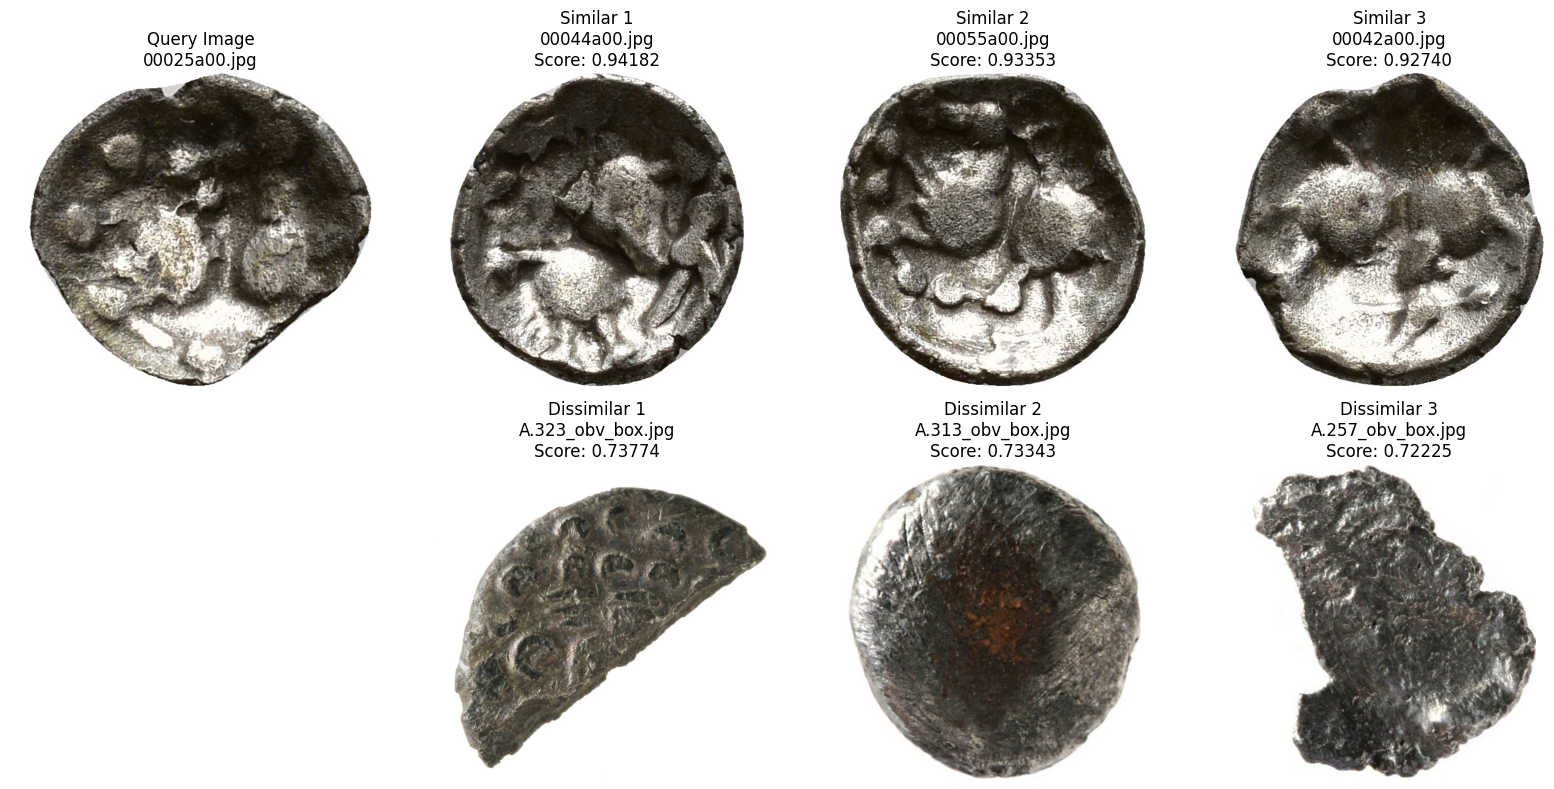
\includegraphics[width=0.8\textwidth]{static/image_similarity_example_1.png}
    \caption{Example 1: Similarity retrieval using image-only embeddings.}
    \label{fig:image_similarity1}
\end{figure}

\begin{figure}[H]
    \centering
    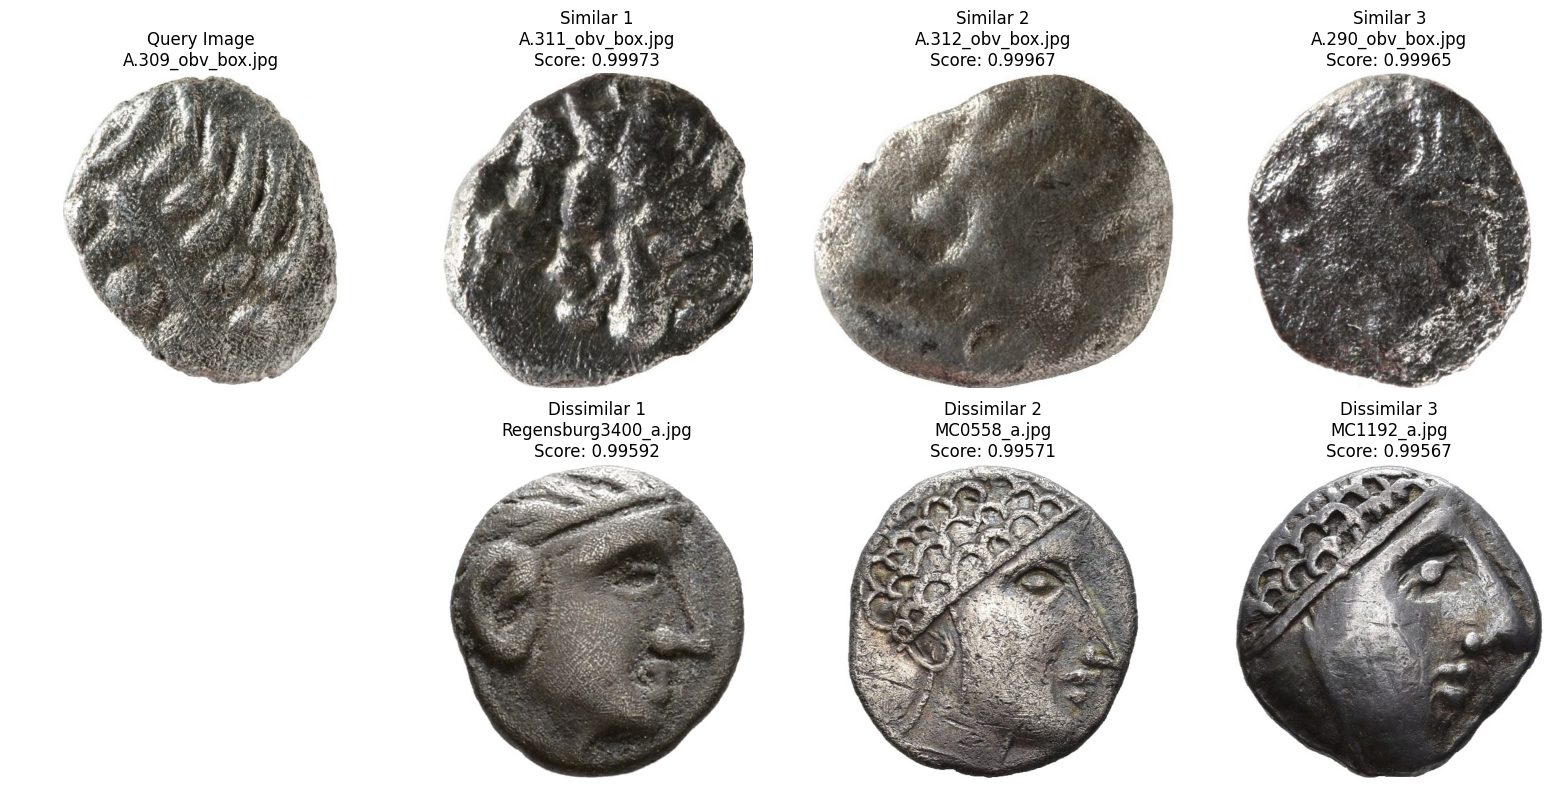
\includegraphics[width=0.8\textwidth]{static/fused_similarity_example_2.png}
    \caption{Example 2: Similarity retrieval using fused embeddings (text+image).}
    \label{fig:fused_similarity2}
\end{figure}

\begin{figure}[H]
    \centering
    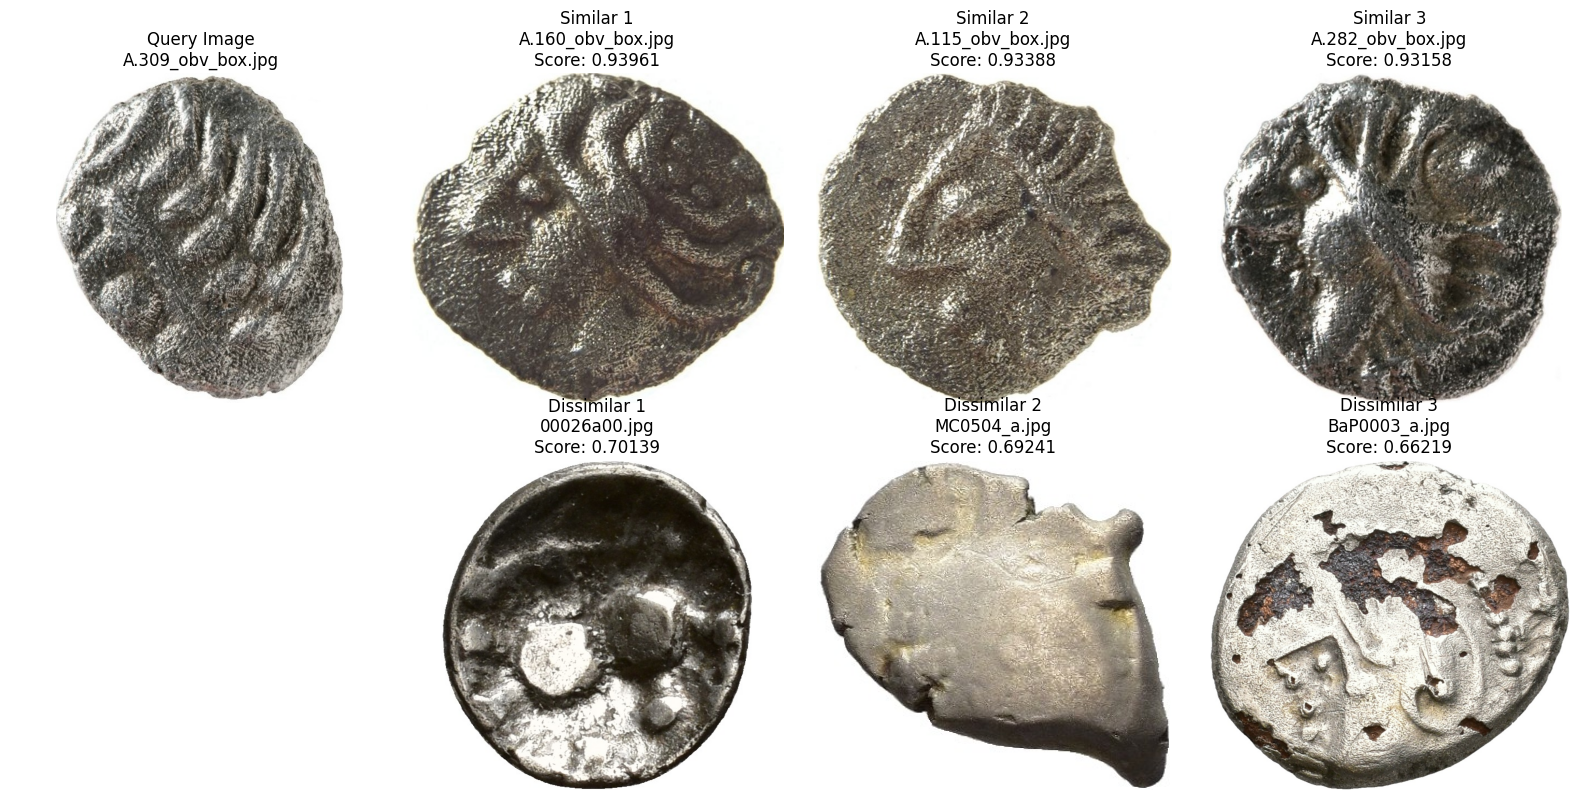
\includegraphics[width=0.8\textwidth]{static/image_similarity_example_2.png}
    \caption{Example 2: Similarity retrieval using image-only embeddings.}
    \label{fig:image_similarity2}
\end{figure}

\begin{figure}[H]
    \centering
    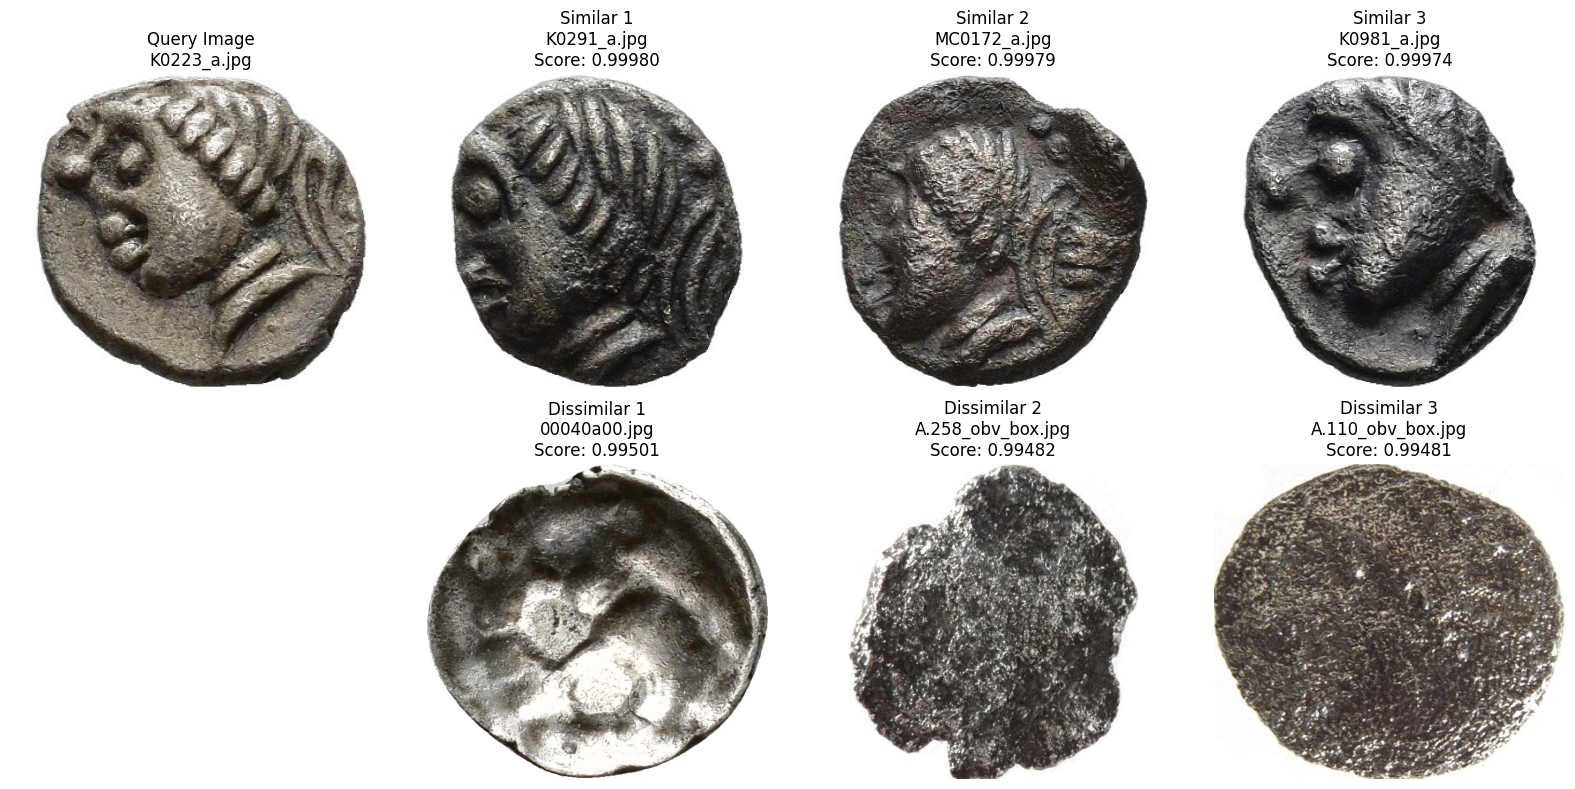
\includegraphics[width=0.8\textwidth]{static/fused_similarity_example_3.png}
    \caption{Example 3: Similarity retrieval using fused embeddings (text+image).}
    \label{fig:fused_similarity3}
\end{figure}

\begin{figure}[H]
    \centering
    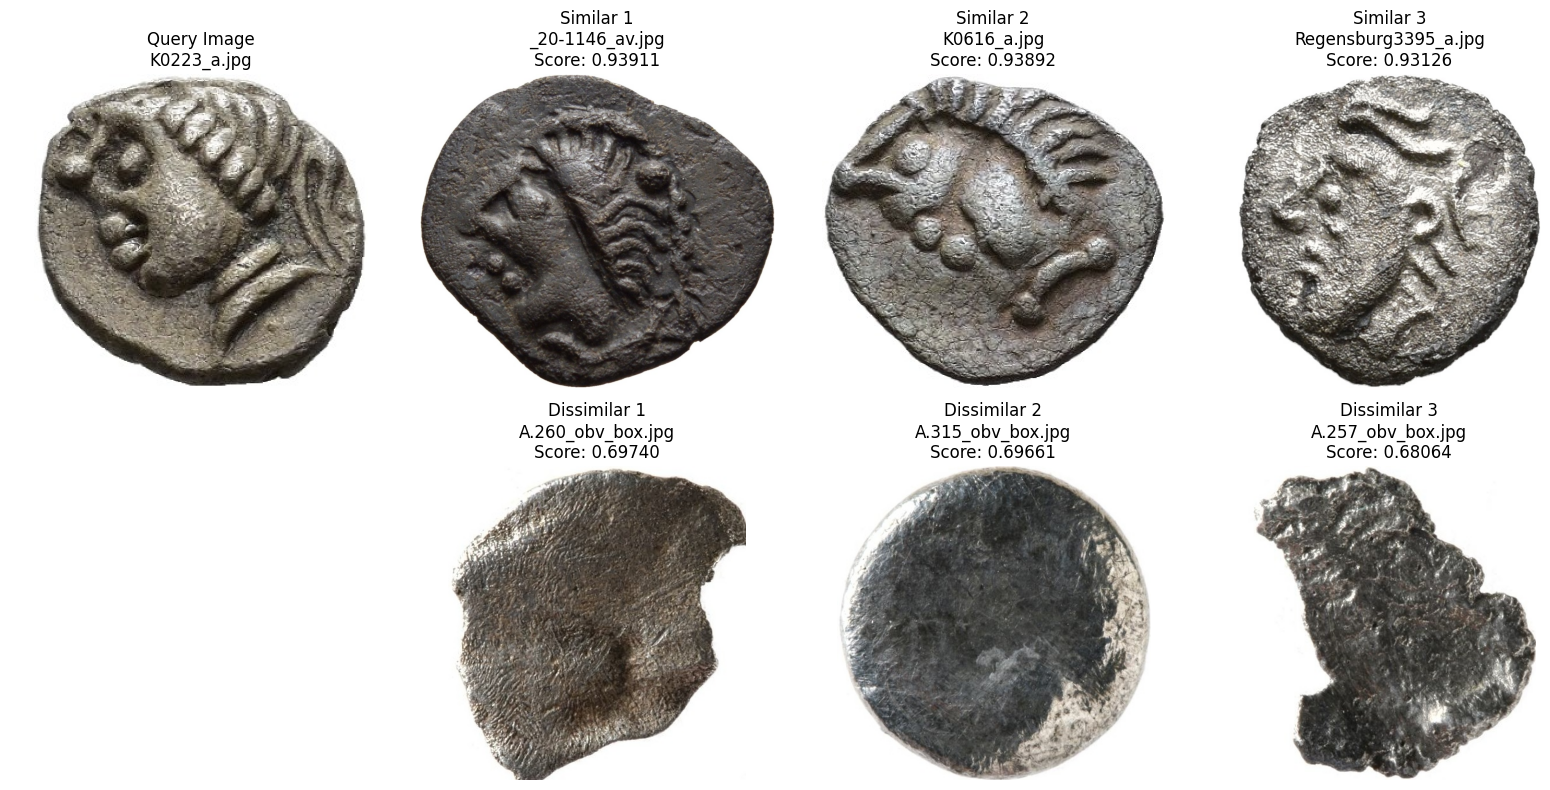
\includegraphics[width=0.8\textwidth]{static/image_similarity_example_3.png}
    \caption{Example 3: Similarity retrieval using image-only embeddings.}
    \label{fig:image_similarity3}
\end{figure}

As observed, the \textbf{multimodal approach produces high similarity scores across all images}, 
sometimes making it difficult to differentiate between similar and dissimilar coins. 
Meanwhile, the \textbf{image-based approach exhibits a more diverse range of similarity values}, 
providing clearer separation between different coin types.

This analysis highlights the impact of incorporating textual information into the embedding space and its effects on 
similarity computations.


\section{Network Analysis of Coin Similarities}
\label{sec:network_analysis}

\subsection{Introduction}
In this section, we analyze the relationships between coin embeddings by constructing a similarity network. 
Each node represents a coin, and edges are drawn between coins whose cosine similarity exceeds a defined threshold. 
This approach helps us understand how coins are clustered based on their visual and multimodal embeddings.

\subsection{Building the Similarity Network}
To construct the network, we used the precomputed embeddings from both the \textbf{ResNet50-based image features} 
and the \textbf{fused CLIP embeddings}. The similarity between two nodes (coins) is determined using cosine similarity. 
If the similarity is above a predefined threshold, an edge is drawn between them.

A major challenge was selecting an appropriate threshold. For image-based embeddings, 
a reasonable threshold (e.g., 0.95) provided meaningful relationships. However, for fused embeddings, 
the similarity values were significantly higher, often exceeding 0.99, making differentiation between coins more difficult.

\subsection{Visualization of Similarity Graphs}
To better interpret the similarity relationships, we generated interactive network graphs. 
These graphs were uploaded to GitHub Pages, allowing for dynamic exploration. 
The following links provide access to the interactive visualizations:

\begin{itemize}
    \scriptsize
    \item \href{https://kenankhauto.github.io/AI-driven-coin-analysis/obverse_fused_graph_0.9995.html}{\texttt{https://kenankhauto.github.io/AI-driven-coin-analysis/obverse\_fused\_graph\_0.9995.html}}
    \item \href{https://kenankhauto.github.io/AI-driven-coin-analysis/reverse_fused_graph_0.9995.html}{\texttt{https://kenankhauto.github.io/AI-driven-coin-analysis/reverse\_fused\_graph\_0.9995.html}}
    \item \href{https://kenankhauto.github.io/AI-driven-coin-analysis/obverse_img_graph_0.95.html}{\texttt{https://kenankhauto.github.io/AI-driven-coin-analysis/obverse\_img\_graph\_0.95.html}}
    \item \href{https://kenankhauto.github.io/AI-driven-coin-analysis/reverse_img_graph_0.95.html}{\texttt{https://kenankhauto.github.io/AI-driven-coin-analysis/reverse\_img\_graph\_0.95.html}}
\end{itemize}

In Figure~\ref{fig:network_image}, we provide an example of a static visualization of the similarity graph.

\begin{figure}[H]
    \centering
    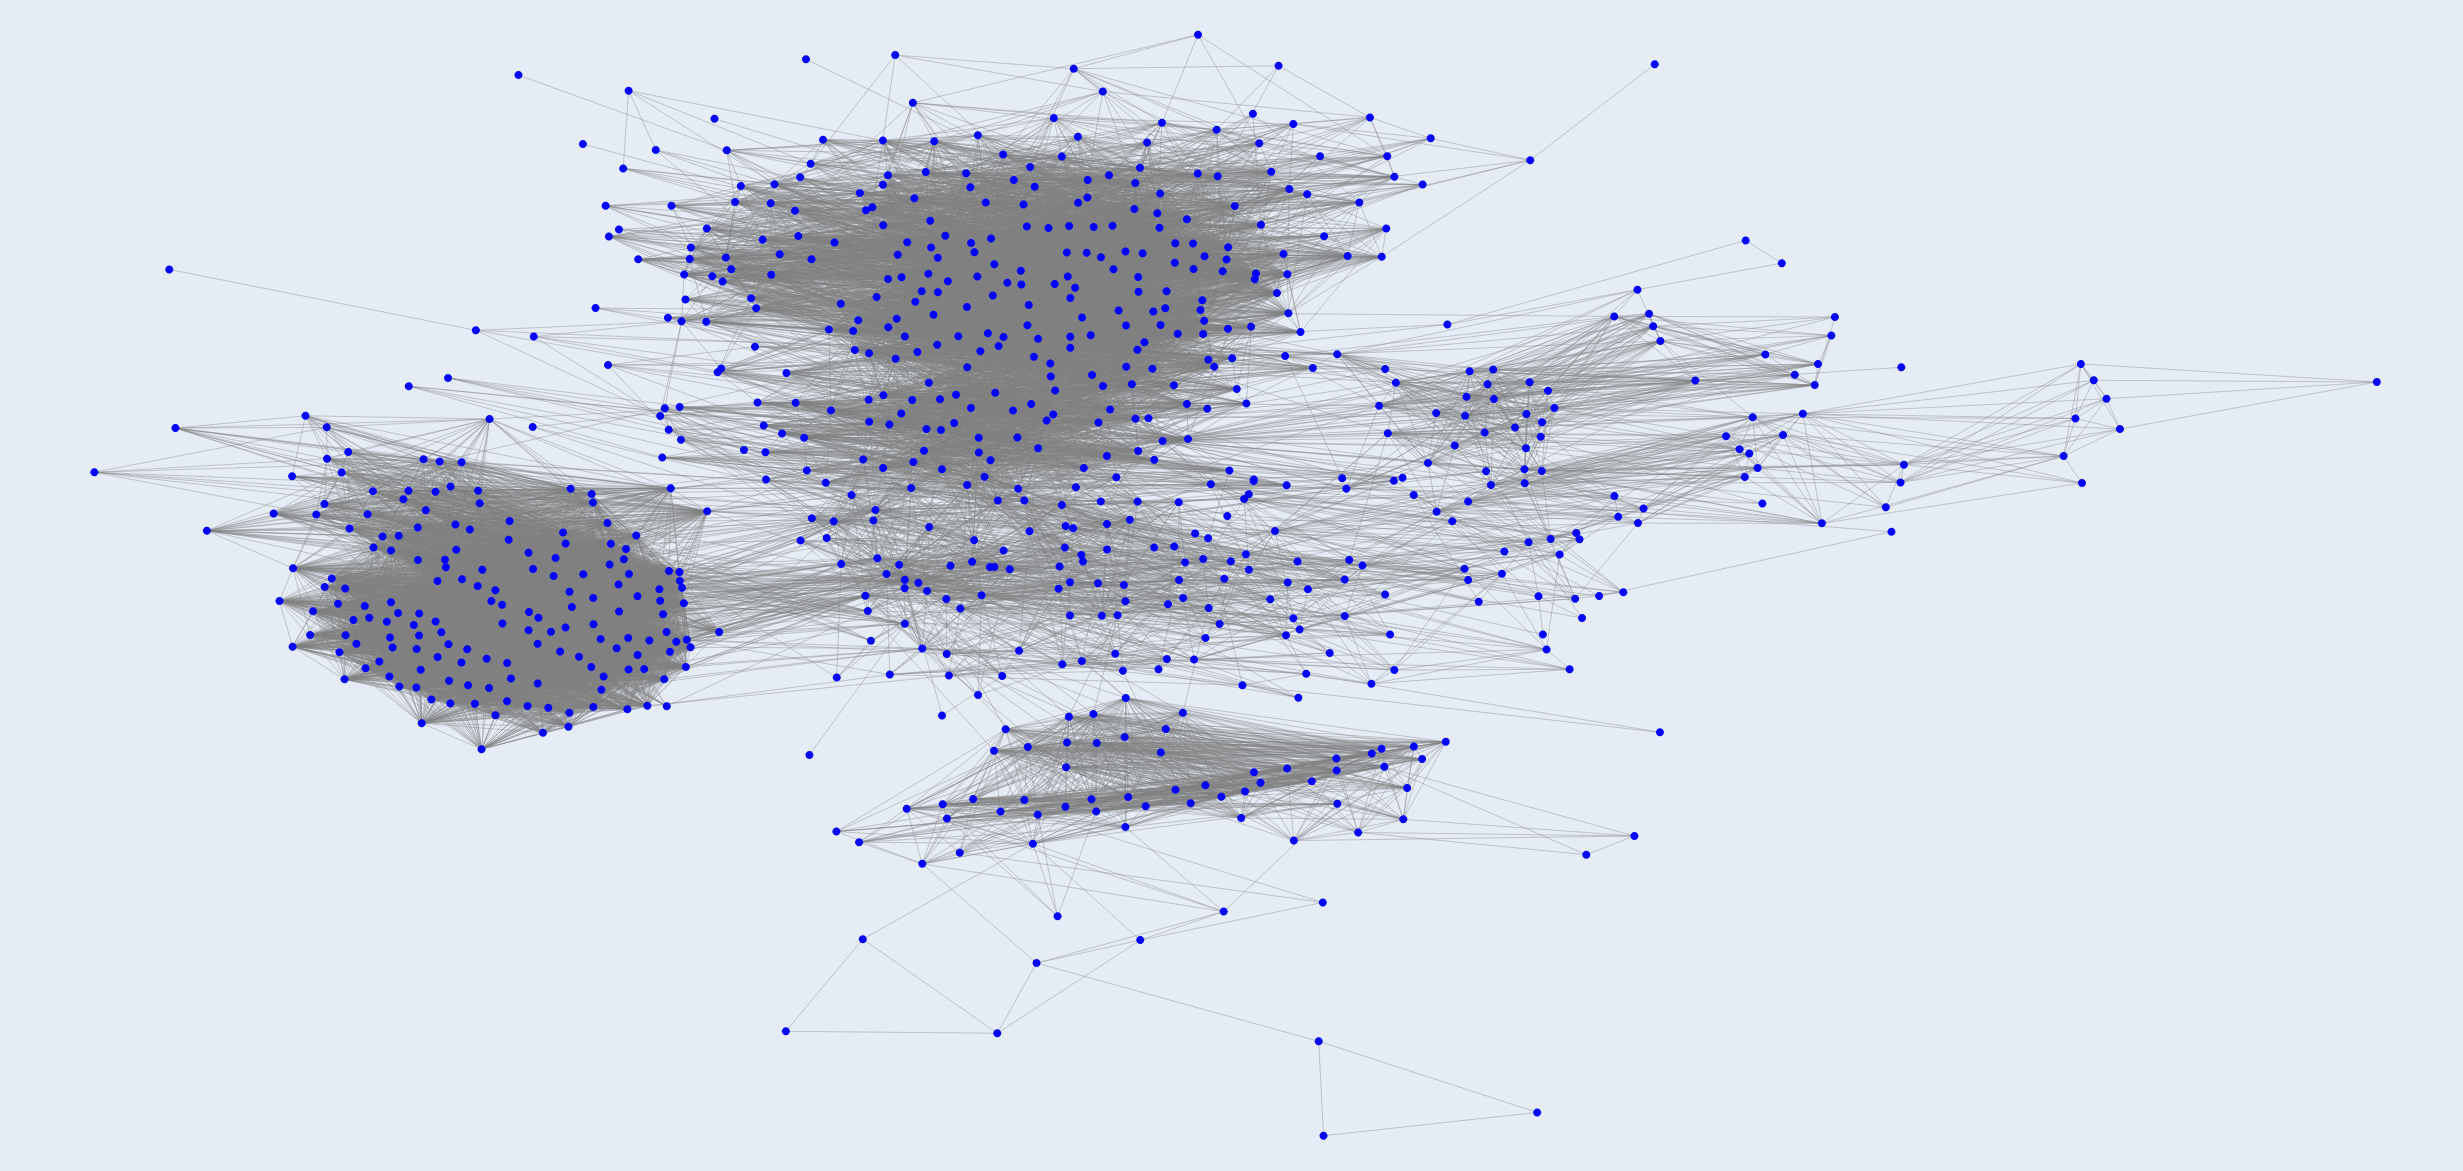
\includegraphics[width=0.85\textwidth]{static/obverse_fused_graph.png}
    \caption{Example of a similarity network for obverse fused embeddings (0.9995).}
    \label{fig:network_image}
\end{figure}

\subsection{Observations}
From the network visualizations, we observe the following:
\begin{itemize}
    \item The \textbf{image-based embeddings} form more distinct clusters, with noticeable separation between different coin types.
    \item The \textbf{fused embeddings} form a denser network, with almost all nodes being interconnected due to 
    the high similarity scores.
    \item Some outlier coins exist, which do not strongly connect to any group.
\end{itemize}

\subsection{Limitations and Challenges}
Despite the insights gained from the network, there are some challenges:
\begin{itemize}
    \item \textbf{Threshold Sensitivity:} A small change in the similarity threshold significantly alters the network structure.
    \item \textbf{High Similarity in Fused Embeddings:} The fused features tend to have artificially 
    high similarity values, making fine-grained distinctions difficult.
    \item \textbf{Lack of Ground Truth:} Since we lack labeled relationships between coins, it is difficult to validate 
    the network against an established classification.
\end{itemize}

\subsection{Conclusion}
The network analysis provided valuable insights into the structure of our coin embeddings. 
The image-based embeddings formed distinct clusters, while the fused embeddings created a more interconnected network. 
These results suggest that multimodal fusion enhances general similarity capture but may require additional 
fine-tuning to differentiate similar yet distinct coins.


\chapter{Evaluation}
Evaluating the performance of the proposed feature extraction and similarity retrieval methods is essential 
to assess their effectiveness in distinguishing and grouping numismatic objects. The evaluation aims to analyze 
the quality of the extracted features, the impact of multimodal fusion on similarity retrieval, and the overall 
performance in retrieving semantically relevant coins.

This chapter is structured as follows:
\begin{itemize}
    \item In Section~\ref{sec:tsne_eval}, we revisit the \textit{t-SNE visualization} of extracted embeddings to 
    observe clustering behaviors and analyze the feature space.
    \item Section~\ref{sec:similarity_retrieval} provides a quantitative analysis of \textit{similarity retrieval}, 
    comparing the performance of image-only embeddings with multimodal fused embeddings.
    \item Section~\ref{sec:limitations} discusses the main issues we observed, and potential solutions.
    \item Finally, Section~\ref{sec:evaluation_summary} summarizes key findings and discusses their implications for 
    numismatic image analysis.
\end{itemize}

The primary goal of this evaluation is to determine whether the fusion of image and text embeddings improves retrieval 
performance and whether the extracted features can effectively cluster similar coin types while maintaining meaningful 
separability among different categories.

\section{t-SNE Feature Space Evaluation}
\label{sec:tsne_eval}

To evaluate the structure of the extracted feature space, we employ 
\textit{t-Distributed Stochastic Neighbor Embedding} (t-SNE) \cite{van2008visualizing}, a widely used dimensionality 
reduction technique for visualizing high-dimensional data. The t-SNE plots help us understand whether the extracted 
features exhibit meaningful clustering and separability.

\subsection{Analysis of Image-Based Embeddings}
\label{subsec:tsne_image}

In previous sections, we generated t-SNE plots for the embeddings extracted using a pretrained ResNet-50 model. 
As shown in Figures~\ref{fig:gray_obverse_tsne} and \ref{fig:gray_reverse_tsne}, the distribution of image-based features 
does not exhibit clear, well-defined clusters. While some local grouping is observable, there is a significant overlap between 
different coin types, indicating that image-based embeddings alone are not highly discriminative for certain coin classes.

This lack of strong clustering suggests that visual features alone may not be sufficient to capture the 
semantic differences between numismatic objects. In cases where coins have similar visual characteristics, 
the embeddings may fail to differentiate between distinct categories.

\subsection{Analysis of Fused Image-Text Embeddings}
\label{subsec:tsne_fused}

In contrast, the t-SNE plots for the fused image-text embeddings, displayed in 
Figures~\ref{fig:tsne_obverse} and \ref{fig:tsne_reverse}, show a remarkable improvement in clustering quality. 
Compared to the image-only features, these embeddings form well-separated and compact clusters, 
indicating that incorporating textual descriptions significantly enhances the feature space's semantic organization.

The improved clustering demonstrates that the multimodal fusion successfully leverages textual descriptions to refine 
feature representation. Coins with similar textual annotations tend to be placed closer in the embedding space, leading to a 
more meaningful grouping. This highlights the advantage of combining both visual and textual information to improve coin 
classification and retrieval tasks.

\subsection{Key Observations}
\label{subsec:tsne_observations}

Based on the visual analysis of the t-SNE projections, the following key insights can be drawn:
\begin{itemize}
    \item \textbf{Image-based embeddings} show moderate clustering tendencies but lack strong separation, leading to ambiguous 
    feature representations.
    \item \textbf{Fused multimodal embeddings} produce well-defined and compact clusters, demonstrating improved feature discrimination.
    \item The incorporation of textual descriptions reduces feature overlap and strengthens the semantic meaning of embeddings, 
    making them more robust for similarity-based retrieval.
\end{itemize}

These findings highlight the importance of leveraging textual information in conjunction with visual features to enhance the 
understanding and classification of numismatic objects.


\section{Similarity Retrieval Performance}
\label{sec:similarity_retrieval}

In this section, we evaluate the similarity retrieval performance of both 
\textbf{image-only embeddings} and \textbf{fused text-image embeddings}. 
The goal of this analysis is to determine how well each embedding method retrieves semantically similar 
coins and whether the inclusion of textual features improves the retrieval process.

\subsection{Retrieval Using Image-Only Embeddings}
\label{subsec:image_retrieval}

For image-based retrieval, we computed cosine similarity between the extracted features using the ResNet-50 model. 
The top-3 most similar and top-3 least similar images were retrieved based on similarity scores.

As seen in Figure~\ref{fig:image_similarity1}, Figure~\ref{fig:image_similarity2}, and Figure~\ref{fig:image_similarity3}, 
the image-only embeddings provided reasonable similarity retrieval results. 
The retrieved images often shared strong \textbf{visual similarities} with the query image, 
such as texture, and overall structure. 

However, one key observation is that this method struggled to recognize \textbf{different stylistic variations of the same coin type}. 
For example, heavily worn coins of the same type appeared visually different and were not always retrieved as the most similar images. 
Additionally, the dissimilar images had noticeably lower similarity scores, demonstrating that the model effectively separated 
different classes.

\subsection{Retrieval Using Fused Image-Text Embeddings}
\label{subsec:fused_retrieval}

By incorporating textual descriptions into the embeddings, 
we aimed to enhance the retrieval process by introducing \textbf{semantic understanding} 
beyond pixel-level similarity. The retrieval was performed using multimodal embeddings obtained from the MLP fusion 
of CLIP text and image features.

As shown in Figure~\ref{fig:fused_similarity1}, Figure~\ref{fig:fused_similarity2}, and Figure~\ref{fig:fused_similarity3}, 
the fused embeddings successfully retrieved images that were semantically closer based on the textual descriptions. 
This allowed the retrieval of coins that shared common symbols and historical attributes, 
even if they had noticeable visual differences.

However, one drawback was observed: \textbf{similarity scores were consistently high, even for dissimilar images}. 
This suggests that while the textual information contributed useful context, it also introduced noise, possibly due to 
the template-based text descriptions. As a result, even when retrieving highly dissimilar coins, 
the similarity scores remained above a certain threshold, reducing the relative contrast between similar and dissimilar items.

\subsection{Comparison of Both Approaches}
\label{subsec:comparison_retrieval}

The comparison between both retrieval methods reveals key trade-offs:

\begin{itemize}
    \item \textbf{Image-only embeddings} produced more reliable visual similarity scores and effectively separated different classes but struggled with stylistic variations of the same type.
    \item \textbf{Fused embeddings} provided better \textit{semantic} retrieval, identifying coins of the same type even when visually different, but suffered from high similarity scores even for dissimilar items.
\end{itemize}

These observations suggest that while multimodal fusion enhances contextual understanding, further refinement is needed to ensure that the retrieved similarity scores reflect true semantic distances.

\section{Limitations and Error Analysis}
\label{sec:limitations}

While the proposed multimodal embedding approach significantly enhances similarity retrieval by 
integrating textual and visual features, it also introduces several limitations that must be addressed. 
This section discusses the key challenges encountered during the study.

\subsection{Influence of Template-Based Text Embeddings}
\label{subsec:text_template_bias}

One of the primary limitations of the fused embeddings is the reliance 
on \textbf{predefined text templates} for generating textual descriptions. 
Although these templates ensure a structured format for textual input, 
they may inadvertently introduce bias into the embeddings.

Since all textual descriptions follow a similar structure (e.g., ``This is the obverse of an ancient Celtic coin depicting [Type]''), 
the model may learn to associate common textual patterns rather than actual semantic differences. 
This can lead to an artificial increase in similarity scores for coins that share generic words in their descriptions, 
even if their visual features are distinct.

\textbf{Potential Solution:} Future work could explore dynamic text descriptions by integrating additional 
metadata (e.g., historical context, minting techniques) or employing generative models to produce richer textual descriptions.

\subsection{High Similarity Scores for Dissimilar Images}
\label{subsec:high_similarity_issue}

As observed in Section~\ref{sec:similarity_retrieval}, the similarity scores for multimodal embeddings 
tend to be consistently high, even for visually dissimilar images. This is particularly evident when comparing the 
least similar images retrieved using image-only embeddings (which show a clear drop in similarity scores)
versus the fused embeddings, where the score differences are minimal.

\textbf{Possible Causes:}
\begin{itemize}
    \item CLIP embeddings naturally encode semantic meaning, which may result in over-smoothing similarity values.
    \item The text embeddings contribute additional information but may overpower fine-grained visual differences.
    \item The concatenation-based fusion method may not fully capture complementary details from both modalities.
\end{itemize}

\textbf{Potential Solution:} Instead of directly concatenating features, alternative fusion techniques 
such as \textit{attention-based mechanisms} or \textit{modality weighting} could be explored to ensure that the image and text 
contributions are balanced.

\subsection{Challenges in Handling Unclassified Coins}
\label{subsec:unclassified_coins}

A subset of the dataset consists of images that lack a predefined type classification. 
Since these images do not have a textual description, they do not benefit from the advantages of multimodal fusion 
and rely solely on visual similarity.

The absence of textual context can lead to incorrect retrieval results when using fused embeddings, 
as these images are mapped differently in the embedding space. This issue highlights the need for a fallback mechanism 
when text information is unavailable.

\textbf{Potential Solution:} A hybrid retrieval system could be implemented, where images without textual descriptions 
default to image-only similarity computations while retaining the option to incorporate text if classifications become 
available in the future.

\subsection{Limitations of the Current Evaluation Metrics}
\label{subsec:evaluation_limits}

The evaluation relied on \textbf{cosine similarity} as the primary metric for retrieval performance. 
While this method is widely used in embedding-based similarity tasks, it has certain drawbacks:
\begin{itemize}
    \item It does not directly account for \textbf{class separability} in the feature space.
    \item Similarity scores do not necessarily correspond to perceptual similarity.
    \item A lack of ground truth labels for all images makes it difficult to compute traditional classification metrics such 
    as precision and recall.
\end{itemize}

\textbf{Potential Solution:} Future work could integrate clustering-based evaluation metrics 
(e.g., \textit{Silhouette Score, Davies-Bouldin Index}) to assess how well the embeddings separate distinct types. 
Additionally, collecting expert-labeled similarity data would enable a more rigorous quantitative evaluation.

\subsection{Impact of Image Preprocessing Choices}
\label{subsec:image_preprocessing}

Finally, image preprocessing steps such as grayscale conversion and normalization influence feature extraction 
and similarity computations. Since CLIP was originally trained on full-color images, converting coins to grayscale may have 
caused a loss of discriminative color-based features.

\textbf{Potential Solution:} A comparative study could be conducted to evaluate performance differences between color and 
grayscale embeddings, ensuring that preprocessing choices align with the optimal use of CLIP.

\subsection{Summary of Limitations and Future Directions}
\label{subsec:limitations_summary}

To summarize, the main limitations identified in this study include:
\begin{itemize}
    \item Bias introduced by template-based text descriptions.
    \item High similarity scores, even for visually distinct images.
    \item Challenges in handling unclassified coins.
    \item Constraints of cosine similarity as a retrieval metric.
    \item Potential loss of information due to image preprocessing.
\end{itemize}

Future research should explore advanced fusion techniques, alternative evaluation methods, 
and dynamic text embeddings to address these challenges and further improve the accuracy of multimodal coin similarity retrieval.


\section{Summary of the Evaluation}
\label{sec:evaluation_summary}

This chapter evaluated the effectiveness of different embedding approaches for coin similarity retrieval. 
We analyzed both \textbf{image-based} and \textbf{multimodal fused} embeddings, comparing their ability to 
cluster similar coins and retrieve relevant matches.

\textbf{Key observations:}
\begin{itemize}
    \item \textbf{t-SNE visualizations} (\ref{fig:tsne_obverse}, \ref{fig:tsne_reverse}) demonstrated that 
    fused embeddings exhibit clearer clustering compared to image-only embeddings, indicating better semantic separation.
    \item While fused embeddings improved retrieval of relevant matches, they also exhibited \textbf{overly high similarity scores}, 
    even for dissimilar images (\ref{fig:fused_similarity1}, \ref{fig:fused_similarity2}).
    \item Template-based text embeddings may have contributed to similarity distortions, 
    as discussed in Section~\ref{subsec:text_template_bias}.
    \item Cosine similarity proved useful for comparing embeddings, but alternative metrics or additional clustering 
    techniques could further enhance evaluation.
\end{itemize}

Despite the limitations identified in Section~\ref{sec:limitations}, the overall results suggest 
that multimodal embeddings can significantly improve numismatic research by enabling automated similarity retrieval. 
However, further refinement of text templates and fusion strategies is necessary to reduce similarity distortions.

The next chapter will provide a \textbf{final conclusion} and discuss possible directions 
for \textit{future research}, including methods for improving embedding quality and incorporating 
additional metadata into the analysis.


\chapter{Conclusion and Future Work}
\label{chap:conclusion}

\section{Summary of Contributions}
\label{sec:summary_contributions}

This study explored the application of \textbf{multimodal embeddings} for numismatic coin similarity retrieval. 
We proposed a novel approach that combines \textbf{image and text embeddings} using CLIP and an \textbf{MLP-based fusion network}, 
allowing for improved similarity detection compared to image-only methods.

The key contributions of this thesis include:
\begin{itemize}
    \item A novel dataset processing pipeline that extracts coin types from structured folders.
    \item The use of a Pretrained-Resnet50 for visual coin representation.
    \item The use of CLIP embeddings for both textual and visual coin representation.
    \item A custom template-based text embedding strategy to describe numismatic images.
    \item The fusion of text and image features via an MLP network, enhancing retrieval.
    \item The use of network analysis techniques to investigate structural relationships between coin similarities.
    \item A detailed evaluation comparing similarity retrieval across different embedding types.
\end{itemize}

\section{Key Findings}
\label{sec:key_findings}

Our experiments led to the following conclusions:
\begin{itemize}
    \item The fused embeddings provided better clustering in 
    \textbf{t-SNE visualizations} (\ref{fig:tsne_obverse}, \ref{fig:tsne_reverse}), 
    showing that text information contributes valuable semantic meaning.
    \item Image-based embeddings alone struggled to form clear clusters, indicating that visual features alone may not be 
    sufficient for nuanced coin classification.
    \item Similarity retrieval using fused embeddings performed well but sometimes exhibited overly high similarity scores,
    even for visually distinct images (\ref{fig:fused_similarity1}, \ref{fig:image_similarity1}).
    \item Text templates played a crucial role but may have introduced \textbf{bias}, 
    which impacted the similarity results (\ref{subsec:text_template_bias}).
\end{itemize}

These findings suggest that multimodal fusion enhances similarity retrieval in numismatics but requires refinement to 
handle textual biases and over-similarity.

\section{Limitations of the Study}
\label{sec:limitations_conclusion}

While this study presents significant advancements, there are still limitations:
\begin{itemize}
    \item \textbf{Limited dataset size}: The study was conducted on a specific numismatic dataset. 
    Testing on a larger dataset could provide more robust conclusions.
    \item \textbf{Textual bias from templates}: The predefined templates may not always reflect the exact historical or 
    artistic significance of each coin.
    \item \textbf{High similarity scores}: The fused embeddings tend to produce very high similarity scores even 
    for dissimilar images, potentially reducing retrieval effectiveness.
    \item \textbf{Lack of ground truth labels}: Due to the absence of exact similarity ground truth, 
    evaluation relied primarily on visualization and relative similarity measures.
\end{itemize}

\section{Future Work}
\label{sec:future_work}

To address these limitations, several future directions could be explored:

\subsection{Dynamic Text Embeddings}
Instead of using fixed templates, integrating \textbf{Natural Language Processing (NLP)} techniques such 
as \textbf{large language models (LLMs)} could generate more contextually rich descriptions, improving text embeddings.

\subsection{Advanced Fusion Strategies}
The MLP-based fusion method could be replaced or extended with:
\begin{itemize}
    \item \textbf{Attention-based fusion} mechanisms to better weight important modalities.
    \item \textbf{Graph Neural Networks (GNNs)} to model relationships between coin images more effectively.
\end{itemize}

\subsection{Alternative Similarity Metrics}
While cosine similarity was used in this study, future work could evaluate:
\begin{itemize}
    \item Mahalanobis distance for similarity retrieval.
    \item Learned similarity functions via contrastive learning.
\end{itemize}

\subsection{Incorporating Additional Metadata}
Additional metadata such as:
\begin{itemize}
    \item Minting date and location,
    \item Material composition,
    \item Numismatic provenance,
\end{itemize}
could be integrated to provide a richer multimodal analysis.

\subsection{Expanding Network Analysis}
The graph-based approach for similarity networks could be improved by:
\begin{itemize}
    \item Using community detection algorithms to classify coins into groups.
    \item Applying PageRank or centrality measures to detect historically significant coins.
\end{itemize}

\section{Final Remarks}
\label{sec:final_remarks}

This thesis demonstrated the power of \textbf{multimodal learning} in numismatic research. 
By combining image and text embeddings, we showed that similarity retrieval can be improved significantly. 
However, the results also highlight the need for better text representations, alternative fusion strategies, 
and improved evaluation metrics.

The findings of this study provide a foundation for further research into automated numismatic analysis, 
with potential applications in \textbf{museum collections, archaeological studies, and digital heritage preservation}.

Future work should focus on refining the fusion process, integrating richer metadata, 
and exploring new similarity measurement techniques to enhance the precision and usability 
of AI-driven coin classification systems.


\printbibliography
\end{document}